\documentclass[11pt]{extarticle}

\usepackage[utf8]{inputenc}

\renewcommand{\familydefault}{\sfdefault}
\setlength\parindent{0pt}

\usepackage{sansmath}
\sansmath

\usepackage{microtype}
\usepackage{amsmath}
\usepackage{minted}
\usepackage{breakcites}
\usepackage{amsfonts}
\usepackage{amssymb}
\usepackage{amsthm}
\usepackage{bm}
\usepackage{caption}
\usepackage{subcaption}
\usepackage{bbm}
\usepackage{enumitem}
\usepackage[margin=2.5cm]{geometry}
\usepackage{fancyhdr}
\usepackage{hyperref}
\usepackage{parskip}
\usepackage{listings}
\usepackage{titling}
\usepackage{graphicx}
\usepackage[dvipsnames]{xcolor}
\usepackage[style=authoryear]{biblatex}
\usepackage{upgreek}
\addbibresource{./bibs/Matching.bib}

\newcommand*\ttvar[1]{\texttt{\expandafter\dottvar\detokenize{#1}\relax}}
\newcommand*\dottvar[1]{\ifx\relax#1\else
  \expandafter\ifx\string_#1\string_\allowbreak\else#1\fi
  \expandafter\dottvar\fi}


\usemintedstyle{manni}

\hypersetup{
    breaklinks=true,
    colorlinks=true,
    citecolor=magenta,
    linkcolor=blue,
    % linkcolor=magenta,
    filecolor=magenta,      
    urlcolor=blue,
    % urlcolor=magenta,
}

% Listings env preferences
\lstset{
    basicstyle=\small\ttfamily,
    columns=flexible,
    breaklines=true
}

% Page styling
\makeatletter
\let\thetitle\@title
\let\theauthor\@author
\let\thedate\@date
% \let\thesubtitle\@subtitle
\makeatother

\pagestyle{fancy}
\renewcommand{\headrulewidth}{0pt}
\lhead{\theauthor}
\rhead{\thetitle}
% \lhead{}
% \rhead{}
\lfoot{{\small{}This document is internal to the University of Chicago Department of Statistics.}}
\cfoot{}
\rfoot{\thepage}
\usepackage{lastpage}

% `answer` box: more customizable
\usepackage{tcolorbox}
\tcbuselibrary{breakable}
\newtcolorbox{solution}[1][]
{
  breakable,
  enhanced,
  sharpish corners,
  boxrule     = 0.25mm,
  boxsep      = 5pt,
  left        = 5pt,
  right       = 5pt,
  top         = 0pt,
  bottom      = 5pt,
  parbox      = false,
  colframe    = ForestGreen!30!black,
  colback     = ForestGreen!5,
  coltitle    = white,
  toptitle    = 0pt,
  bottomtitle = 0pt,
  title       = {\bfseries Solution},
  #1,
}

\allowdisplaybreaks

% Shortcuts for math
\newcommand{\reals}{\ensuremath{\mathbbmss R}}
\renewcommand{\vec}[1]{\ensuremath{\boldsymbol{\mathsfbf{#1}}}}
\newcommand{\mat}[1]{\ensuremath{#1}}
\newcommand{\set}[1]{\ensuremath{\mathcal{#1}}}

% Subtitle! https://tex.stackexchange.com/questions/50182/subtitle-with-the-maketitle-page
\newcommand{\subtitle}[1]{%
  \posttitle{%
    \par\end{center}
    \begin{center}\large#1\end{center}
    \vskip0.5em
  }%
}


\title{Development of a Python Package for Matching Observational Data}
\subtitle{Advisors: Jingshu Wang, Sanjay Krishnan}
\author{Jack Potrykus}
\date{\today}

\begin{document}

% Insert some text making clear that this is an MS thesis
\begin{center}{\large \bfseries Master’s Paper for the University of Chicago Department of Statistics}\end{center}

% Relax `\maketitle` to allow text on same page. https://tex.stackexchange.com/questions/86249/maketitle-text-before-title
{\let\newpage\relax\maketitle}


\section*{Abstract}
\label{sec:abstract}

Observational studies are widely used throughout econometrics, psychology, and medical research.
Matching is a field in causal statistics concerned with algorithms to minimize the effect of selection bias in the observational data on analyses of treatment effects.
In particular, in binary treatment/control studies, these algorithms work by matching each treatment observation to one or more ``nearby'' control observations.
This paper breaks the matching procedure down into two key components: how distance is measured, and how matches are assigned.
In doing so, it explores several distance metrics, in particular the propensity score \parencite{rosenbaum_central_1983}, the prognostic score \parencite{hansen_prognostic_2008}, and exact matching \parencite{iacus_causal_2012} and its machine learning extensions \parencite{liu_interpretable_2019, wang_flame_2021}; it then explores several matching algorithms that can be used to produce the matched subset once the distance is calculated, in particular the Hungarian algorithm \parencite{munkres_algorithms_1957} and greedy algorithms \parencite{ho_matchit_2011}.
I then showcase the functionality of \texttt{matching}, an open-source Python package I have developed for matching observational data which takes a graph-centric approach, something which no other package offers.
I finally explore some practical considerations of parameter tuning when matching via experiments on simulated data.

% Insert a spot for the advisor's signature
\vfill{\null}
Approved by: \hrulefill~Date: \hrulefill

\newpage{}
\tableofcontents{}
\newpage{}


\section{Introduction}
\label{sec:intro}

Observational studies are of ever-increasing importance as the numerous amount of data collected each year continues to grow.
However, of observational studies are at a major disadvantage compared to blocking-based study design or randomized control trials, because the researchers do not have control over the distribution of confounding variables, known or unknown, in the data itself. As such, researchers must take preliminary steps to alter the data in some way in order to minimize the effects of selection bias, which results from heterogeneous distributions present in the observational data.

Within the field of causal inference, the term \emph{matching} is often associated with observational studies with a binary treatment indicator.
Using a similar framework to that of \textcite{iacus_multivariate_2011}, consider $\mat{X}_T \in \reals^{n \times p}$ and $\mat{X}_C \in \reals^{m \times p}$, matrices of $p$ features for $n$ treatment-group observations and $m$ control-group observations, $n \leq m$.
We seek to produce a matching $\set{M}$ such that each observation in $\mat{X}_T$ is paired with one or more nearby observations from $\mat{X}_C$, according to a distance metric and a matching algorithm.

The choice of distance measure and choice of matching algorithm are orthogonal, and this paper (and the Python package) will discuss them as such. Indeed, measuring distance, as well as \emph{balance diagnostics} between treatment and control distributions, are problems most associated with the field of statistics; in contrast, producing the optimally matched subset is a \emph{minimum cost flow} problem in the field of computer science \parencite{rosenbaum_optimal_1989}.

I then introduce a Python package I have developed, \texttt{matching}, which provides an idiomatic and flexible tool for matching observational data. It achieves this by allowing distance measures and matching algorithms to be independently and iteratively applied, so that even incredibly bespoke matching procedures may be implemented succinctly in code. It is also the first Python library for matching observational data which is ``graph-centric'': the key data structure used is a bipartite graph, whose nodes represent observations, and edge weights the distance measure between them. This enables further exploration into new matching procedures and balance diagnostics using graph metrics and algorithms from computer science.


% Matching algorithms in practice come in two forms


\section{Literature Review}
\label{sec:litrev}


\subsection{Measuring Distance}

In the context of this paper, distance measures are functions $d: \reals^p \times \reals^p \mapsto \reals^+$ which produce a non-negative distance, or ``cost of matching'', between any vectors $\vec{x}_T, \vec{x}_C$ from the rows of $\mat{X}_T \in \reals^{n \times p}$ and $\mat{X}_C \in \reals^{m \times p}$, to judge the match quality. Distance measures are often combined with some preprocessing function $f(\mat{X})$, usually in the form of a dimension reduction or discretization of the data. Again using a framework akin to that of \textcite{iacus_multivariate_2011}, one may succinctly describe a distance measurement as
\begin{equation}
  \mathcal{D}_d (f(\mat{X}_T), f(\mat{X}_C)), \label{eqn:abstractdistance}
\end{equation}
where $\mathcal{D}_d : \reals^{n \times p} \times \reals^{m \times p} \mapsto \reals^{n \times m}$ is a ``vectorized'' version of $d$, producing a matrix $\mat{D}$ whose $(i, j)$th element is the distance between observation $i$ from $\mat{X}_T$ and observation $j$ from $\mat{X}_C$.


\subsubsection{Balancing Scores}

Balancing scores
\footnote{Balancing scores come in a variety of forms: as \textcite{rosenbaum_central_1983} note, $b(X) = X$ is the simplest balancing score. However, this paper uses the term ``balancing score'' specifically with regards to 1-dimensional reductions of the data. That is to say, that we will consider balancing scores as a preprocessing function $b: \reals^{(n + m) \times p} \mapsto \reals^{n + m}$.}
\parencite{rosenbaum_central_1983} are a versatile class of functions $b(X)$ satisfying the property
\begin{equation}
  \mat{X} \perp \vec{z} | b(\mat{X}), \label{eqn:defbalancingscore}
\end{equation}
where the matrix $\mat{X} \in \reals^{(n + m) \times p} = \mat{X}_T \cup \mat{X}_C$, and the vector $\vec{z} \in \reals^{n + m}$ contains binary treatment group assignments.
In words, given the balancing scores $b(\mat{X})$, the distribution of the feature matrix $\mat{X}$ is independent of treatment assignment $\vec{z}$. These methods each set $d$ equal to the $L^1$ norm, or absolute distance, by convention. In the notation of~\eqref{eqn:abstractdistance}, then, balancing scores compose the class of distance measures of the form
\begin{equation}
  \mathcal{D}_{L^1}(b(\mat{X})_T, b(\mat{X})_C).
\end{equation}

Balancing scores afford observational data some of the desirable properties of randomized trials. Namely, in a randomized trial, $\mat{X}$ should contain all features used in determining treatment assignment, affording conditional independence of outcomes from treatment:
\begin{equation}
  \vec{y}_0, \vec{y}_1 \perp \vec{z} | \mat{X}, \label{eqn:defstrongignorable}
\end{equation}
where $\vec{y}_0$ and $\vec{y}_1$ are vectors of outcomes, for which the $i$th element is the outcome of observation $i$ when assigned to group 0 (control) or 1 (treatment); note that in practice we almost always only observe $y_{0,i}$ \emph{or} $y_{1,i}$ for each $i$. If the statement in~\eqref{eqn:defstrongignorable} holds, then the treatment assignment is \emph{strongly ignorable}. \textcite{rosenbaum_central_1983} then prove that if~\eqref{eqn:defstrongignorable} holds (that is, treatment $\vec{z}$ is strongly ignorable given features $\mat{X}$), then treatment assignment is \emph{also} strongly ignorable given any balancing score $b(X)$! Conditioning on balancing scores, we gain independence of treatment from features, as well as the strong ignorability of treatment; these useful properties form the key motivation for the use of balancing scores in causal inference.


\paragraph{The Propensity Score.} In the same paper, \textcite{rosenbaum_central_1983} propose the balancing score $b(\mat{X}) = \mathbbmss E \left [\vec{z} | \mat{X}\right ]$, also known as the propensity score.
This is simply a predicted probability (or logit) that any given feature vector $\vec{x} \in \mat{X}$ belongs to the treatment group.
This is the most prevalent balancing score in the literature, and indeed the most prevalent distance measurement overall. It is almost always estimated by logistic or probit regression \parencite{garrido_methods_2014}, but other classifiers are possible.
By preprocessing $\mat{X}$ to a single dimension of scores $b(\mat{X})$, we not only reduce computation time necessary for $\mathcal{D}$, but also implicitly apply a weighting to the feature matrix $\mat{X}$: the features most predictive of treatment assignment (i.e., most heterogeneous between the two groups) will be the most closely matched. \cite{dehejia_causal_1999} evaluated the performance of propensity score methods, and found that, given the assumption that treatment depends only on pre-intervention observable features, propensity score methods can serve as a useful diagnostic, particularly for examining the degree of ``overlap'' in feature distributions between the two groups.

\paragraph{Extensions of the Propensity Score.} Acknowledging that propensity score methods have thus far been limited to binary, multinomial, or ordinal treatment assignments in the literature (as they are considered in this paper), \textcite{imai_causal_2004} explored extensions of the propensity score into the realm of quantitative treatments. In their paper, they consider the treatment vector \emph{packyear}, the number of packs smoked by a smoker each year, and subclass the resulting scores into a varying number of bins. They found that conditioning on the subclass helped to reduce bias by between 16\% and 95\%.

\paragraph{The Prognostic Score.} \textcite{hansen_prognostic_2008} discussed the \emph{prognostic score}, a balancing metric on outcomes. The only difference between the construction in~\eqref{eqn:defbalancingscore} is that we exchange $\vec{z}$ for $\vec{y}$, a vector of outcomes.
\begin{equation}
  \mat{X} \perp \vec{y} | b(\mat{X}) \iff b \text{ is a prognostic balancing score} \label{eqn:prognosticscoredef}
\end{equation}
The prognostic score is constructed nearly in exactly the same way as the propensity score; however, in order to preserve~\eqref{eqn:prognosticscoredef}, the model (linear/logistic regression, random forest, etc.) is trained on the \emph{control data alone}. This model is then used to predict scores over the \emph{whole dataset}.

The idea of using outcomes, either raw or ``preprocessed'', does not see unanimous support; \textcite{garrido_methods_2014} argues against incorporating any information about outcome into the matching process. \textcite{miettinen_stratification_1976} was a seminal paper in matching that used outcome stratification; this method has since been found to be suboptimal, and has been effectively replaced by prognostic scores and other methods \parencite{hansen_bias_2006} (Miettinen's ``multivariate confounder score'' used the \emph{full} dataset, not just the control, when fitting). \textcite{hansen_bias_2006} argues for its inclusion via a ``conditionality principle'', which suggests that if some statistic (in this case, $b(\mat{X})$) is known to be uninformative about the parameter being estimated (i.e. treatment effects), it should be included in inferential models.

\textcite{stuart_prognostic_2013} found prognostic scores to be highly correlated with bias in estimates of treatment effects, and thus a useful diagnostic tool, even when the model was misspecified. Thus, prognostic scores can serve as a useful ``proxy'' for the reduction in bias of the estimates. Nonetheless, they also caution that their use in matching depends on the researcher's appetite to reduce the separation of data identification and analysis of outcomes in their study.

\paragraph{Joint Use of Balancing Scores.} \textcite{leacy_joint_2014} further explores of calculating \emph{both} propensity and prognostic scores, stratifying each into a $p \times p$ grid, and considering observations within each of the $p^2$ grid squares as a \emph{matched strata}. However, they found that matching on prognostic scores alone performed the best, while matching on propensity scores and Mahalanobis distance (see \S\ref{subsubsec:normdist}) also performed admirably. The $p \times p$ strata performed better than stratification of either score alone, but could not beat matching on either un-discretized score alone. They also found that the percent bias of estimates created using this matching method increased with the non-linearity in the outcomes model.

\paragraph{Calipers.} Propensity and prognostic scoring methods often add one more hyperparameter: a \emph{caliper}, $c$. The caliper is used to calculate \emph{caliper width}, equal to the product of $c$ and the standard deviation of the scores \parencite{ho_matchit_2011}.
The caliper serves to establish a radius of acceptable matches around each observation's propensity score as a form of quality control: if the observations are too dissimilar (their distance is greater than the caliper width), then they may not match.
This comes with a cost: if the caliper is sufficiently small, observations with outlying feature vectors $\vec{x}$ may not have any suitable matches, and the matched subset remaining for treatment effect analyses may be substantially smaller.

\textcite{austin_optimal_2011} explored the question of choosing an optimal caliper width under a variety of regimes. When all features were iid Gaussian random variables, calipers $c \in [0.05, 0.15]$ maximized the reduction in bias, with each reduction on the order of $98.9\%$ or greater. \citeauthor{austin_optimal_2011} then introduced correlation when generating the feature matrix, as well as including a varying number of independent $\text{Bernoulli}(0.5)$. Under the correlated regime, the optimal caliper varied between $0.05$ and $0.30$, depending on the true risk reduction given the generated features. However, he also notes that the percent bias reduction decreased as the number of Bernoulli features increased, and that when \emph{all} features were Bernoulli-distributed, the choice of caliper had no effect on bias reduction.

\paragraph{Criticism.} The most notable criticism of balancing score based distance measurement comes from \textcite{king_why_2019}. King and Nielsen's argument is twofold: first, from an experimental design perspective, they argue that \emph{fully blocked} study design, which other distance measures attempt to emulate (in particular: Mahalanobis distance, Coarsened Exact Matching), dominates \emph{complete randomization study design}, which balancing-score based methods attempt to emulate.
Whereas each study design balances unobserved confounding features on average, fully blocked methods assure balance of observed confounding features, whereas complete randomization only promises balance \emph{on average}.
They thus regard balancing score methods as having a ``lower standard''.
Second, they observe the ``Paradox of Propensity Score Matching'': consider the case where $\mat{X} \perp \vec{z}$, and so all predicted scores are the same constant: $\hat{\vec{z}}$.
Then, all potential matches are indecipherable, and the individual matchings may be complete nonsensical, and in fact may \emph{increase} the imbalance of features within the matched subset. The authors nonetheless concede that propensity scores (and other balancing scores, by extension) do indeed have nice theoretical properties, and may serve as a useful diagnostic; they contend only that they should not be used for matching.

\subsubsection{Exact Matching and Almost Exact Matching}
\label{subsubsec:exactmatching}

Among other methods which seek to replicate fully blocked study design, \textcite{king_why_2019} argue for ``coarsened exact matching'', or CEM. This requires the researcher to first preprocess their data into discrete categories: for example, a vector ``age'' might be grouped into buckets. They then suggest exact matching on the now-discretized features into \emph{strata}, and applying observational weights to the data according to the formula
\begin{equation}
  w_{i}= \begin{cases}1, & i \in \text{treatment group} \\ \frac{m_{C}}{m_{T}} \frac{m_{T}^{s}}{m_{C}^{s}}, & i \in \text{control group} \end{cases},
\end{equation}
where $w_i$ denotes the observation weight for observation $i$, $m_T$ and $m_C$ are the total number of matched treatment and control observations, and $m_T^s$ and $m_C^s$ are the total number of matched treatment and control observations \emph{within observation $i$'s stratum, $s$} \parencite{iacus_causal_2012}.

\textcite{iacus_multivariate_2011} introduces a formal definition for a class of distance measures which they call ``monotonic imbalance bounding'', or MIB. These methods are designed to require no assumptions about the distribution of the data, and to emphasize minimizing \emph{in-sample} imbalance, as opposed to \emph{sample} balance. These methods take a vector of tuning parameters $\vec{\uppi}$, such as a vector of calipers. These methods afford the benefit that the number of matches is a function of the tuning parameters alone, and given monotonicity of the maximum distance function $\gamma_{\mathcal{D}_{d}}(\vec{\uppi})$, can be each adjusted independently other others: if $\gamma$ is vector-valued, the element-wise differences of feature vectors can be independently compared in a system of inequalities. CEM is an example of an MIB distance measure, but this class is clearly much more flexible, allowing for precise adjustments.

\paragraph{Almost Exact Matching.} Some of the most modern methods are DAME \parencite{liu_interpretable_2019} and FLAME \cite{wang_flame_2021}, which incorporate machine-learning generated weight vectors indicating the relative importance of features to extend exact matching into the field of \emph{almost exact matching}. These two algorithms are unified by their tendency to sometimes ``drop'' uninformative features from the matching process, in order to ensure that the most important features are matched on, and potentially increase the number of potential matches. The chief difference can be summarized as follows: DAME choosing a subset of features to match on by minimizing predictive error, whereas FLAME maximizes a match quality statistic that the researcher can tune via a hyperparameter; this statistic is a function of predictive error and a \emph{balance factor}, which represents the relative size of the strata of observations matched on this subset on features \parencite{gupta_dame-flame_2021}.

\subsubsection{$L^p$ Norms and Mahalanobis Distance}
\label{subsubsec:normdist}

Norms of the difference between feature vectors (i.e. $\| \vec{x}_T - \vec{x}_C \|_p$) themselves are usually used in the form of Mahalanobis distance, which first rescales all features to have mean zero and unit variance, and then calculates distances using the $L^2$ norm.
This ensures that all features have equal weight in the matching, which may or may not be desirable; in either case, it almost certainly better than the no-rescaling case, where a feature's variance would determine its relative importance.
As \textcite{king_why_2019} notes, norm-based distance metrics attempt to replicate fully-blocked design, and thus offer some theoretical advantages.
However, many are attracted to the ability of balancing score methods, as well as modern methods such as DAME and FLAME, to discern which features are \emph{most important} to match on. 

Nonetheless, \textcite{leacy_joint_2014} finds Mahalanobis distance to perform well when the number of features was small, each of which was approximately normally distributed. Additionally, many modern matching software packages allow for initially establishing a ``perimeter'' of viable matches using a caliper and a propensity score, and subsequently matching on the Mahalanobis distance between the feature vectors \parencite{ho_matchit_2011}.

\subsubsection{Iterative Distance Calculations}

Often, researchers will employ an ``iterative'' distance measure. They may, for example, first calculate propensity scores $\widehat{\vec{z}}$, filter potential matches using a caliper $c$, and then match on Mahalanobis distance \emph{within} clusters; or, in the absence of a caliper, within strata of $\widehat{\vec{z}}$. This idea was explored by \textcite{rosenbaum_constructing_1985}, who found it to perform better than matching on either propensity score or Mahalanobis distance alone. 

\textcite{baltar_mahalanobis_2014} explored the efficacy of this iterative method in practice, relative to propensity score and Mahalanobis distance alone. In the paper, they compare seek to estimate the effect of Brazilian towns' social agenda on public health. They found both the propensity score alone and iterative method to perform admirably, whereas Mahalanobis distance performed poorly; they do not take this as an indictment of Mahalanobis distance matching, and pose for further research to identify conditions under which Mahalnobis distance may perform \emph{better}. The iterative method achieved the greatest reduction in bias for all features, except the propensity score, for which propensity score distance alone (somewhat obviously) saw the greatest bias reduction. However, as \textcite{austin_optimal_2011} and \textcite{greifer_assessing_2022} note, balance of the scores does not imply balance of the features, and balancing score balance metrics should only be used as a supplementary diagnostic; the focus of balance assessment should be balance of the features.

\subsection{Matching Algorithms}

Once the distance measure has been agreed upon, the researcher must then decide \emph{how} to match. A computer scientist could describe this problem as finding the minimum weight full matching of a \emph{bipartite graph}, whose nodes represent observations, and whose edge weights represent the distance between them. Here, the term ``bipartite'' means that all edges in the graph map $T \leftrightarrow C$; within each disjoint subset, no two nodes share an edge. This paper will explore the optimal solution to this problem in both the $1:1$ and $1:k$ matching scenarios, as well as fast approximations.


\subsubsection{Optimal Matching}

\textcite{rosenbaum_optimal_1989} argues for optimal matching according to the Hungarian algorithm, also known as the Kuhn-Munkres or simply Munkres algorithm \parencite{munkres_algorithms_1957}. We will denote a matching a set $\set{M}$ of tuples $(i, j)$, with $i$ representing a treatment-group observations, and $j$ a control-group observations. The Hungarian algorithm solves the \emph{linear assignment problem}, which in this setting may be expressed as
\begin{equation}
  \min_{\set{M}} \sum_{(i, j) \in \set{M}} d(\vec{x}_{T_{i}}, \vec{x}_{C_{j}}), \text{ such that } \forall (i, j), (k, l) \in \set{M}, i = k \iff j = l;
\end{equation}
the ``such that'' condition simply specifies that the matching is one-to-one. As such, optimal matching via the Hungarian algorithm minimizes the total sum of distances between matches in the matched subset.

\paragraph{Extensions.} The Hungarian algorithm can be extended to the $1:k$ matching case via $b$-matching while retaining optimality.
This process involves adding $k$ ``copy'' nodes for each node representing a $T$ datapoint, each with identical edges as the original node, and then perform the optimal matching on the resulting graph.
However, as \textcite{khan_efficient_2016} notes, this can lead to calculations which quickly become time consuming as the total number of data points increases. \textcite{khan_efficient_2016} goes on further to explore efficient approximation algorithms of the $b$-matching, such as the $b$-\textsc{Suitor} algorithm.

\subsubsection{Greedy Matching}

Greedy algorithms have the benefit of running much quicker than optimal matching algorithms, and are often the default in other observational data matching software, such as \texttt{MatchIt} \parencite{ho_matchit_2011}. These methods are equivalent to sorting the edges of the graph in ascending order, and naively popping off the top of the list the next match. While these methods benefit from speed, they guarantee nothing with regards to optimality. This can be particularly problematic in the $1:k$ scenario \parencite{rosenbaum_optimal_1989}, where the order in matches are assigned can have matches implications; compare this to optimal matching, which is a simultaneous match.

\subsection{Balance Assessment}

Researchers may wish to assess the balance of their matching, particularly when attempting to heuristically optimize a hyperparameter, such as the caliper. Common numerical methods include standardized mean-differences, variance ratios, and empirical CDF (eCDF) comparison between the two groups \parencite{greifer_assessing_2022}. Most researchers do not check for convergence of moments beyond the second, and as \textcite{basu_use_2008} report, these moments exhibit much slower convergence, the effects of which can be particularly detrimental when outcome depends on some non-linear function of the joint distribution of $\mat{X}$. For this reason, \textcite{zhu_kernel-based_2018} recommend using density-based metrics, such as total variation distance or Kolmogorov-Smirnov distance. It is also important to note that balance of the $i$th moment does not imply balance of the $j$th moment across the two groups for $j \geq i$ \parencite{garrido_methods_2014}.

There are also many graphical diagnostics for assessing balance. QQ-plots, eCDFs, and density estimates for for the unmatched data and the matched subset, perhaps overlaid, effectively visually convey the balance improvement from matching. One may also plot the improvement in standardized mean differences between the two groups, referred to as a Love plot \parencite{greifer_assessing_2022}. One could also plot the bipartite graph to understand where clusters are appearing, or how large groups of ``similar'' observations are, or which observations are most ``dissimilar'' from the rest.


\section{\texttt{matching}: a Python Package for Matching Observational Data}

The most popular implementation of bipartite matching for observational studies is the \texttt{MatchIt} package for R \parencite{ho_matchit_2011}.
The GitHub repository\footnote{\url{https://github.com/kosukeimai/MatchIt}} boasts an impressive $37000$ downloads per month, and with good reason: the authors of the package are also authors of many of the most popular papers in the field of matching (e.g. \textcite{ho_matching_2007, imai_causal_2004, king_why_2019, stuart_matching_2010}).

\texttt{MatchIt} is largely used through a single function: \texttt{Matchit::matchit}, which minimally accepts a \texttt{formula} (like those used in \texttt{lm}), \texttt{data}, and a \texttt{method}. The function also allows for iterative matching procedures, complex filters on the suitability of potential matches, and a selection of bipartite matching algorithms. The output of the function is furthermore easily inspected via the ubiquitous \texttt{summary} function, or plotted via \texttt{plot}.

However, R is not as popular ``in-industry'' as it once was. Whereas academics have largely favored R as their programming language of choice, Python has become the \emph{lingua franca} of data scientists. The TIOBE index\footnote{\url{https://www.tiobe.com/tiobe-index/}} currently lists Python as the most popular programming language in the world, with nearly ten times the market share of R.
It is then surprising that there is no package for matching observational data that is as flexible and feature-complete as \texttt{MatchIt}. This is what lead me to developing \texttt{matching}, a Python library for matching observational data.

\subsection{Design Goals}

After exploring \texttt{MatchIt}'s capabilities, as well as the Python landscape of matching packages for causal inference, I set out to create a package that is:
\begin{itemize}
  \item inspectable. The user should be able to numerically and graphically inspect each step of the matching procedure.
  \item flexible. The package should provide ``plug-and-play'' tools to customize and conduct an arbitrarily complex matching procedure, without the user needing to implement new classes.
  \item familiar. The package should mimic idioms from popular data science packages\footnote{e.g. \texttt{numpy}, \texttt{pandas}, \texttt{sklearn}, \texttt{networkx}}, and all outputs should be easily coercible to a \texttt{pandas.DataFrame} or a \texttt{numpy.ndarray} for further analysis.
  \item ``depth over breadth''. The package should only implement matching procedures, leaving model-building and effect estimation to the user; narrowing in on the matching procedure alone also helps to achieve the first three goals.
\end{itemize}
In particular, I focused on separating responsibility between how the distance between feature vectors is calculated, and how the matches are then assigned. Being able to easily adjust distance measure and matching procedure independently is especially valuable when assessing the matching quality via diagnostic tools when tuning a hyperparameter, e.g. the maximum allowable distance, or the number of matches $k$ to find for each treatment observation.

\subsection{Architecture}

The package is organized into the following modules.
\begin{itemize}
  \item \texttt{matching.balance}: implementations of common balance measures, such as standardized mean difference, variance ratio, and eCDFs.
  \item \texttt{matching.dataset}: implementation of the \texttt{MatchingDataset} class, which parses user data into an easily manageable format.
  \item \texttt{matching.distance}: the \texttt{\_Distance} base class and concrete implementations of distance measures, such as \texttt{Norm}.
  \item \texttt{matching.graph}: the \texttt{MatchingGraph} class implementation; this is the main class that the user interacts with.
  \item \texttt{matching.graph\_utils}: functional graph utilities.
  \item \texttt{matching.preprocessing}: functional preprocessing utilities, such as propensity scoring, prognostic scoring, and auto-coarsening.
\end{itemize}

Most users will only need to use \texttt{matching.graph} and \texttt{matching.distance}, perhaps in addition to some light preprocessing with \texttt{matching.preprocessing} as necessary.
These two submodules represent the algorithmic matching, and distance calculations separately.
This separation of responsibility into two separate class hierarchies allows for high flexibility in the matching procedure, as each component can be changed independent of the other.

\begin{figure}[h!]
  \center{%
    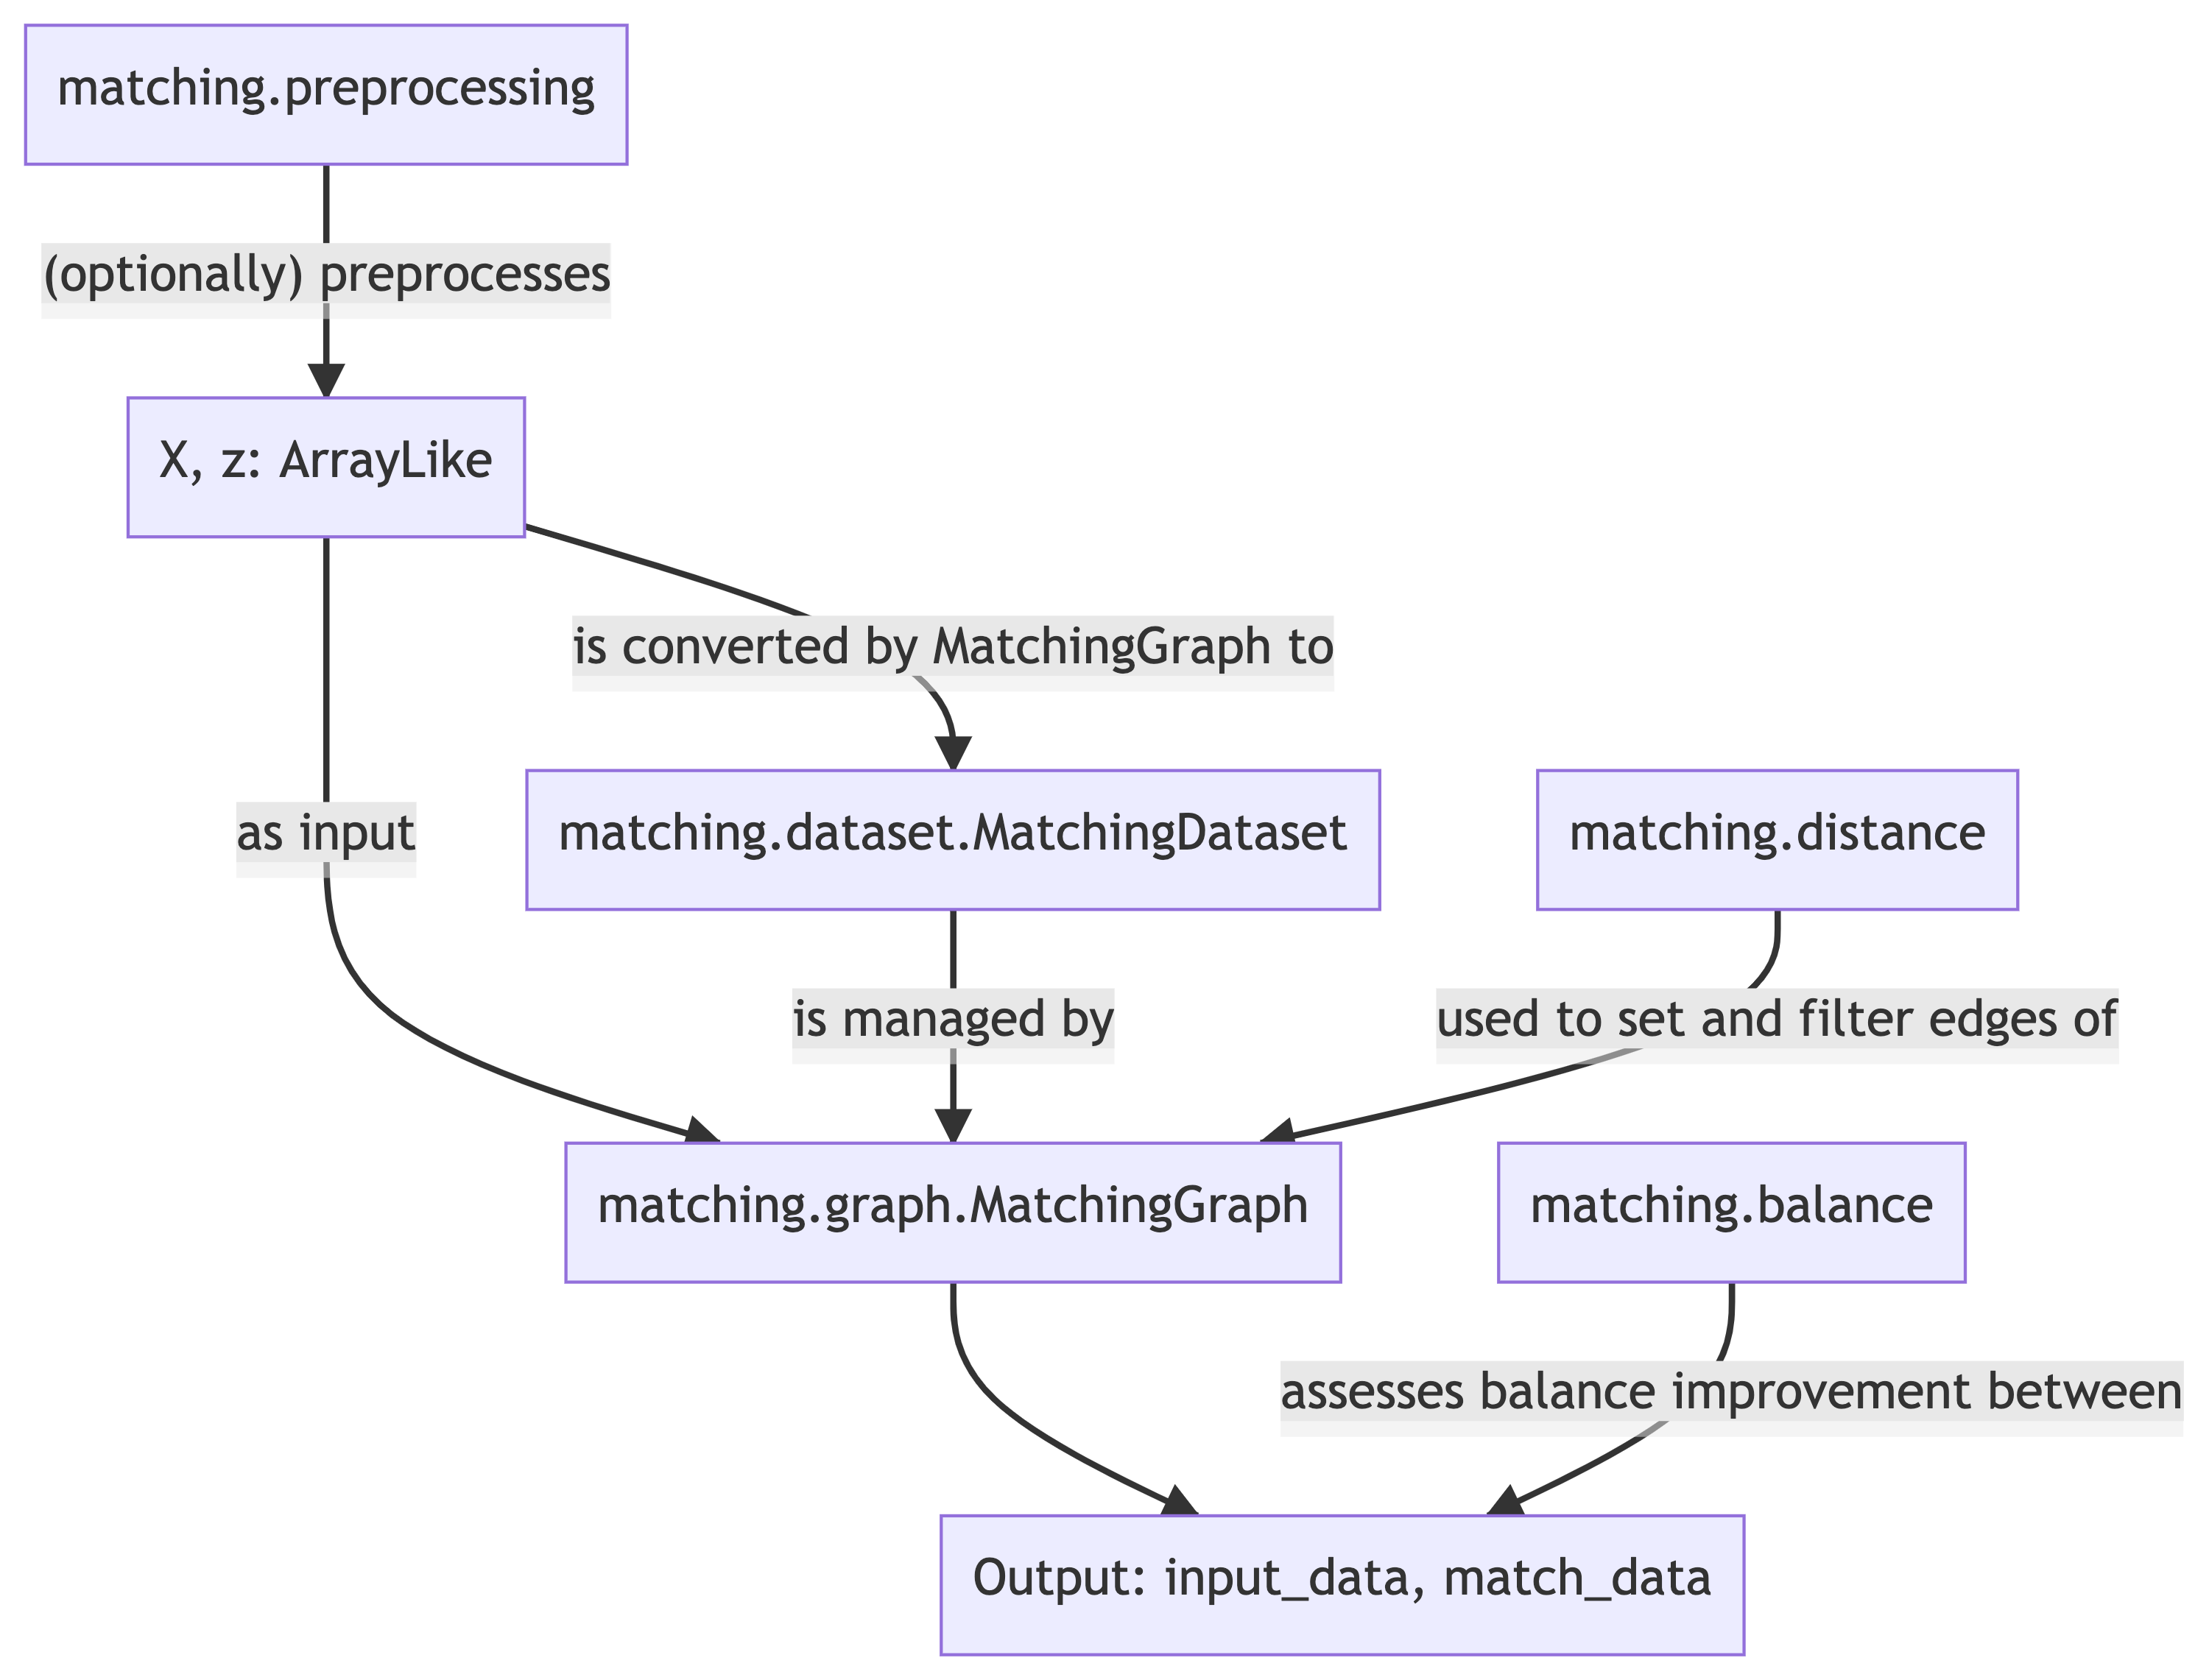
\includegraphics[width=0.8\textwidth]{../docs/mermaid/img/relationships.png}%
  }
  \caption{\label{fig:arch_flow} The relationships between the different modules of \texttt{matching}}.
\end{figure}

\begin{figure}[h!]
  \center{%
    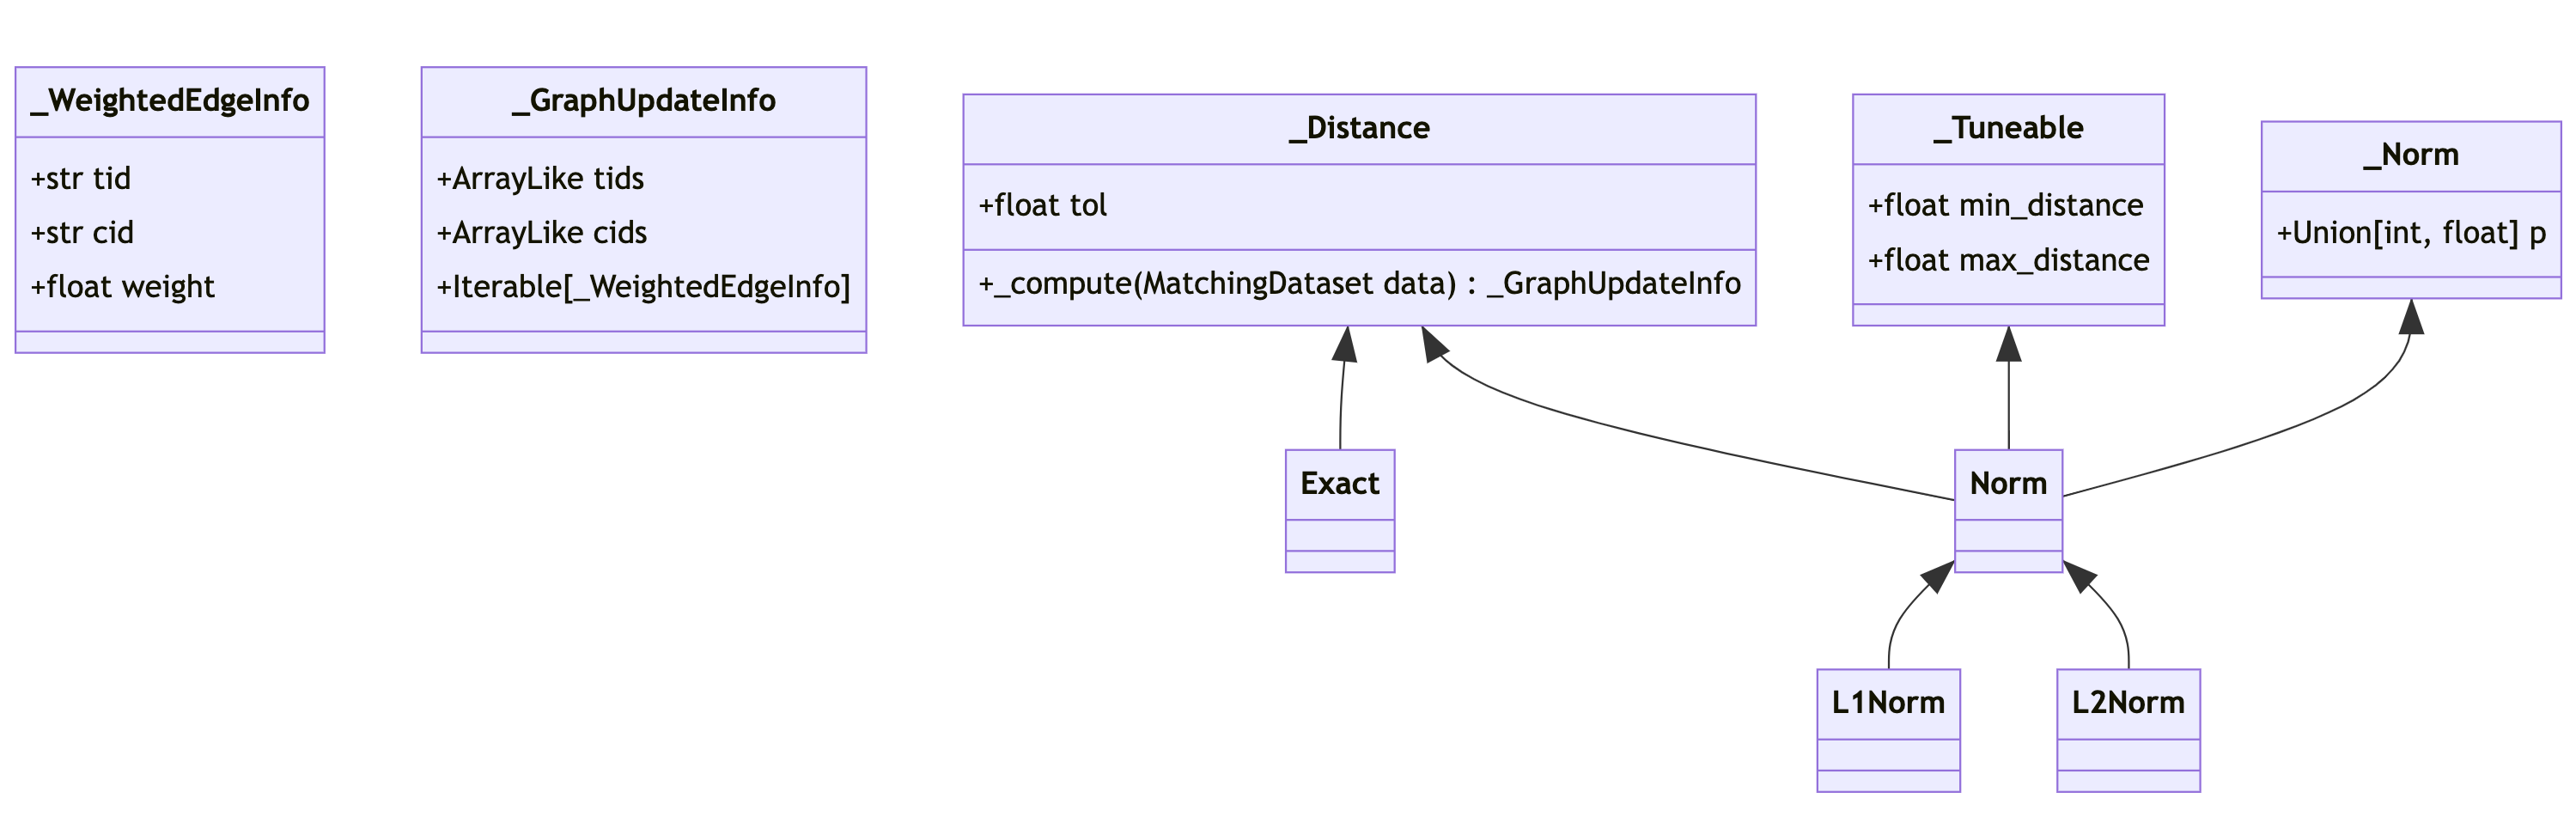
\includegraphics[width=\textwidth]{../docs/mermaid/img/distance_uml.png}%
  }
  \caption{\label{fig:distance_uml} UML Diagram for the \texttt{matching.distance} submodule}
\end{figure}

\newpage
\subsection{Usage}
\label{subsec:usage}

Typical usage of the \texttt{Matching} package is outlined in Figure~\ref{fig:matching_usage}. A written explanation of each step follows.

\begin{figure}[h!]
  \center{%
    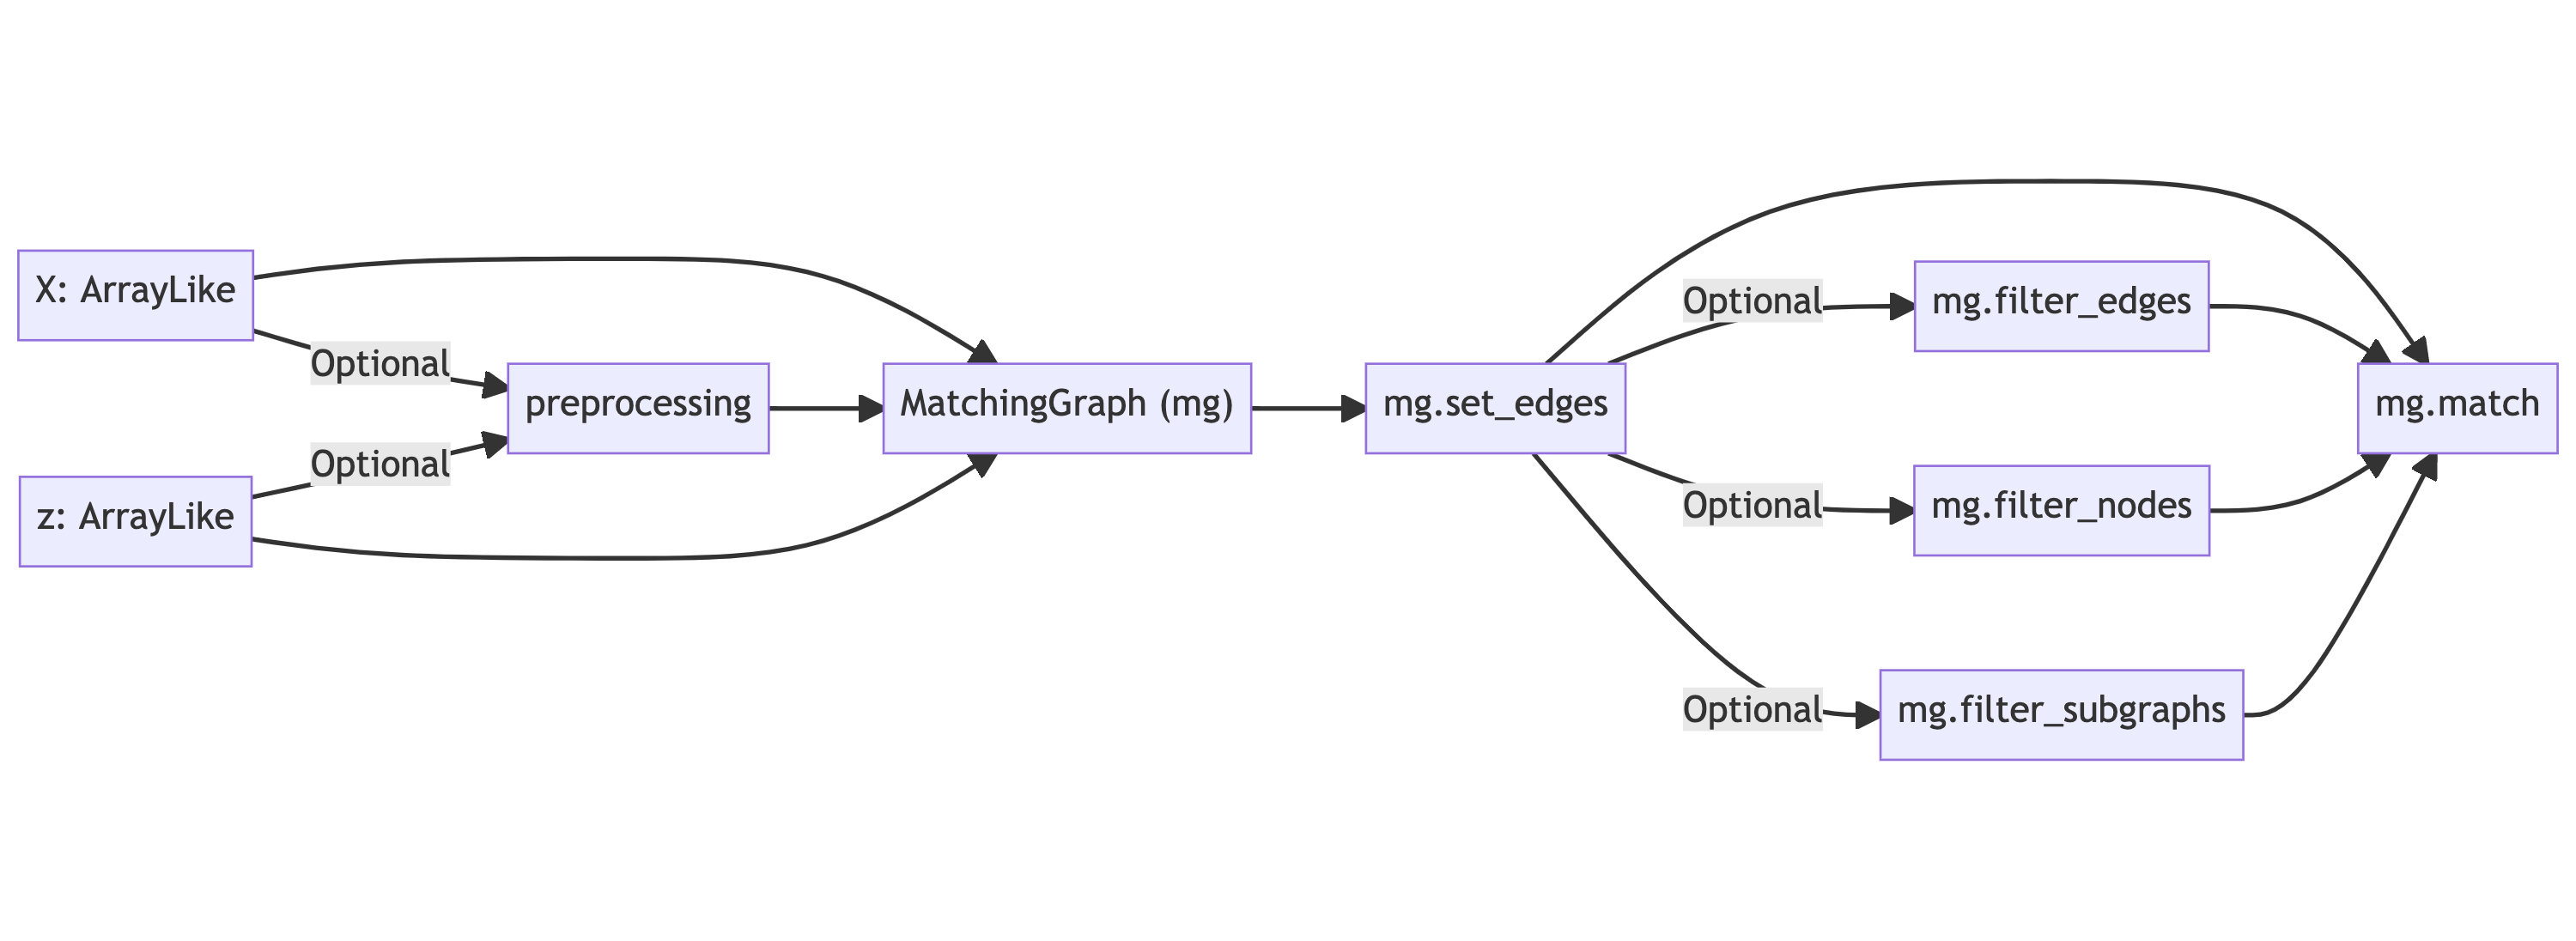
\includegraphics[width=\textwidth]{../docs/mermaid/img/usage_flow.png}%
  }
  \caption{\label{fig:matching_usage} Flow diagram describing typical usage of the \texttt{matching} package}
\end{figure}

\paragraph{Initialization.} 
The \texttt{MatchingGraph} is minimally initialized with an array-like (e.g., a \texttt{pandas.DataFrame}, or a \texttt{numpy.ndarray}) of features \texttt{X} and an array-like of binary treatment assignments \texttt{z}. The user may first wish to preprocess their data (e.g. calculating propensity scores) using \texttt{matching.preprocessing}, but this is not necessary.
\begin{minted}[linenos, fontsize=\small]{python3}
from matching.graph import MatchingGraph
from matching.preprocessing import propensity_score

# Possibly some preprocessing... (not shown)
# X is an array of propensity scores, z is an array of booleans
mg = MatchingGraph(X, z)
\end{minted}
\paragraph{Setting Edges.} The user should then make a call to the \texttt{set\_edges} method to calculate the distance between each observation the two groups, and set the graph nodes and edge weights. Here, the user supplies a \texttt{\_Distance} measure from \texttt{matching.distance}. The user may supply a \texttt{min\_distance} and/or a \texttt{max\_distance} for an edge to be allowed; in graph terms, this can be considered the edges' \emph{capacity}. For the \texttt{PropensityScore} distance metric, \texttt{max\_distance} is instead set by specifying a \texttt{caliper}; the \texttt{max\_distance} is later inferred, once the scores are calculated.
\begin{minted}[linenos, fontsize=\small]{python3}
import numpy as np
from matching.distance import PropensityScore

# Will calculate propensity score distance automatically
mg.set_edges(distance=PropensityScore(caliper=0.05))
\end{minted}
\paragraph{Iterative Filtering.} It is possible to implement iterative distance measures as well. Consider \texttt{X} as a dataframe with columns \texttt{"score"}, containing propensity scores, and \texttt{"is\_nice"}, a boolean series. We would like to match on propensity scores within \texttt{caliper\_width}, but also cannot assign any nice people to any naughty people. We can make use of the \texttt{filter\_edges} method and the \texttt{include} keyword argument to accomplish this.
\begin{minted}[linenos, fontsize=\small]{python3}
from matching.distance import Exact, L1Norm
from matching.graph import MatchingGraph
from matching.preprocessing import propensity_score

# Take caliper_width as given
# X has columns "score" and "is_nice", z is treatment assignments
mg = MatchingGraph(X, z)
# NOTE: there is also a keyword argument "exclude"
mg.set_edges(distance=L1Norm(max_distance=caliper_width), include=["score"])
mg.filter_edges(distance=Exact(), include=["is_nice"])
\end{minted}
The \texttt{filter\_edges} command will drop any potential matches who do not match exactly on \texttt{"is\_nice"} by simply deleting the edge between them. This extends beyond exact-match filtering. One could filter using \texttt{L2Norm}, for instance, to drop potential matches whose $L^2$ norm distance was above some maximum threshold.

There are also methods to \texttt{filter\_nodes} by label or order, as well as to \texttt{filter\_subgraphs}, which filters the disjoint subgraphs of the graph by a variety of metrics\footnote{\texttt{filter\_subgraphs} is particularly relevant for strata-based matching methods like CEM, which often filter strata based on the total number of observations (from each group), the ratio of treatment to control.}; they will not be discussed here, but readers are referred to \texttt{matching} documentation hosted on the GitHub\footnote{\url{https://github.com/jackpotrykus/propensity-score-matching-thesis}}.

\paragraph{Matching.} Once the user has set the edges of the graph and completed their filtering, they may wish to conduct a $1:k$ matching between treatment and control, for some integer $k \geq 1$\footnote{This is not always necessary, particularly in the case of CEM.}
The user does this via a call to the \texttt{match} method. The user can control $k$ with \texttt{n\_match}, the maximum number of matches to find for each observation. Some treatment observations will not be able to be matched with this many control observations; they can be automatically pruned with the \texttt{min\_match} parameter. The parameter \texttt{replace} is a boolean, indicating whether multiple treatment observations may match with the same control observation, which is \texttt{False} by default. Finally, the user has a choice of greedy (keyword argument: \texttt{"greedy"} or \texttt{"fast"}) or optimal matches (keyword argument: \texttt{"optimal"}, \texttt{"hungarian"}, \texttt{"kuhn"}, or \texttt{"munkres"}).
\begin{minted}[linenos, fontsize=\small]{python3}
# Continue from the previous excerpt. Now we want to conduct 1:k matching
# NOTE: By default: n_match=1, min_match=1, replace=False
mg.match(n_match=2, min_match=2, method="optimal")
\end{minted}

\paragraph{Balance Assessment.} The user can then compare the balance of the \texttt{input\_data} and the \texttt{match\_data}\footnote{In the case of Exact matching edges, the \texttt{match\_data} should consist of all subgraphs of order at least 2.}. Note that \texttt{match\_data} is a subset of \texttt{input\_data}, plus a new column, \texttt{"match\_group"}.
\begin{minted}[linenos, fontsize=\small]{python3}
# Can get dataframes of input_data and match_data
input_df = mg.input_data.frame
match_df = mg.match_data.frame

# Assess balance improvement via the MatchingDataset.summary() method
input_balance = mg.input_data.summary()
match_balance = mg.match_data.summary()

# ... or import the balance functions themselves
# Let's compare the eCDF of scores between the input_data and the match_data
from matplotlib import pyplot as plt
import numpy as np
from matching.balance import ecdf

# Fit eCDFs to the scores in each dataframe
input_score_ecdf = ecdf(input_df["scores"])
match_score_ecdf = ecdf(match_df["scores"])

# Evaluate the eCDFs at 101 points between 0 and 1
xs = np.linspace(0, 1, 101)
input_score_ecdf_at_xs = input_score_ecdf(xs)
match_score_ecdf_at_xs = match_score_ecdf(xs)

# Plot them to compare
plt.plot(xs, input_score_ecdf_at_xs)
plt.plot(xs, match_score_ecdf_at_xs)
plt.show()
\end{minted}

\paragraph{Drawing the Graph.} After edges have been set using \texttt{set\_edges}, users may draw the graph at any point in the matching process. \texttt{networkx} provides a myriad of functions to draw graphs, but the \texttt{MatchingGraph} class has two convenient graph-drawing methods built-in. These are the methods \texttt{draw} and \texttt{draw\_bipartite}. The main difference between these two is that \texttt{draw} will draw the graph such that edge length is proportional to the distance between observations, whereas \texttt{draw\_bipartite} draws the graph in the \emph{bipartite layout}, with all treatment group nodes on one side, and all control group nodes on the other. Example output of each of these is displayed in Figure~\ref{fig:draw_examples}.
\begin{figure}[h!]
    \centering
    \begin{subfigure}[t]{0.5\textwidth}
        \centering
        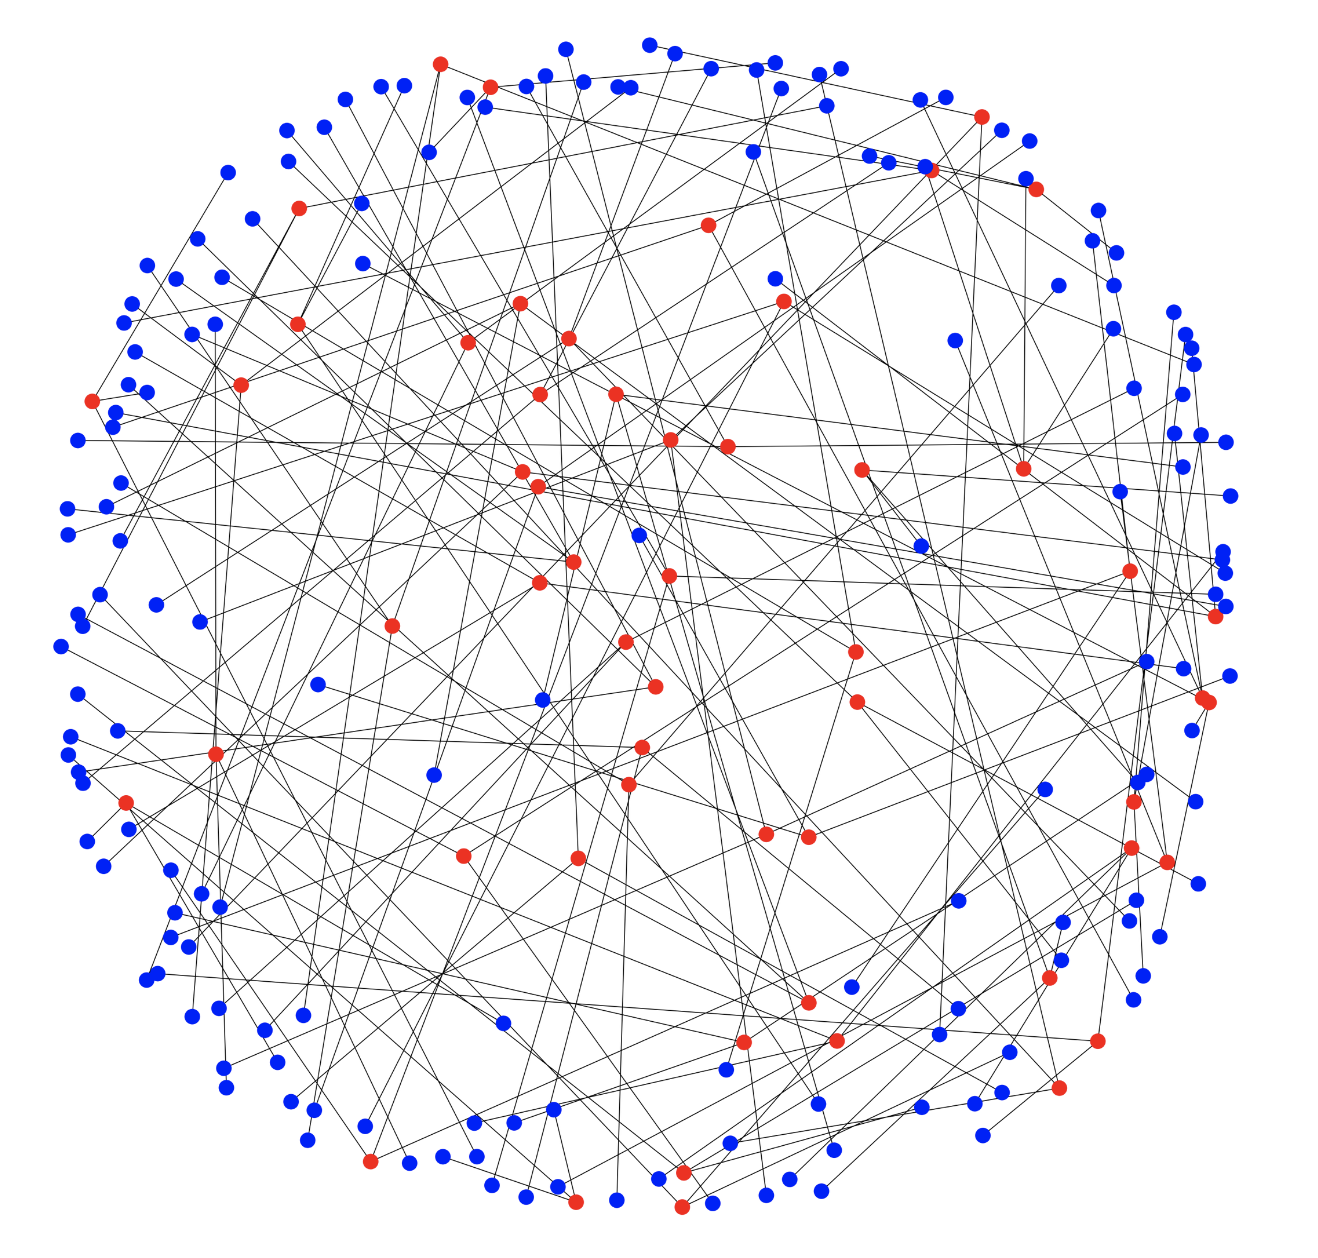
\includegraphics[width=0.95\textwidth]{./img/draw_examples/draw.png}
        \caption{Graph produced by \texttt{mg.draw()}. Edge length corresponds to the distance between observations.}
    \end{subfigure}%
    ~
    \begin{subfigure}[t]{0.5\textwidth}
        \centering
        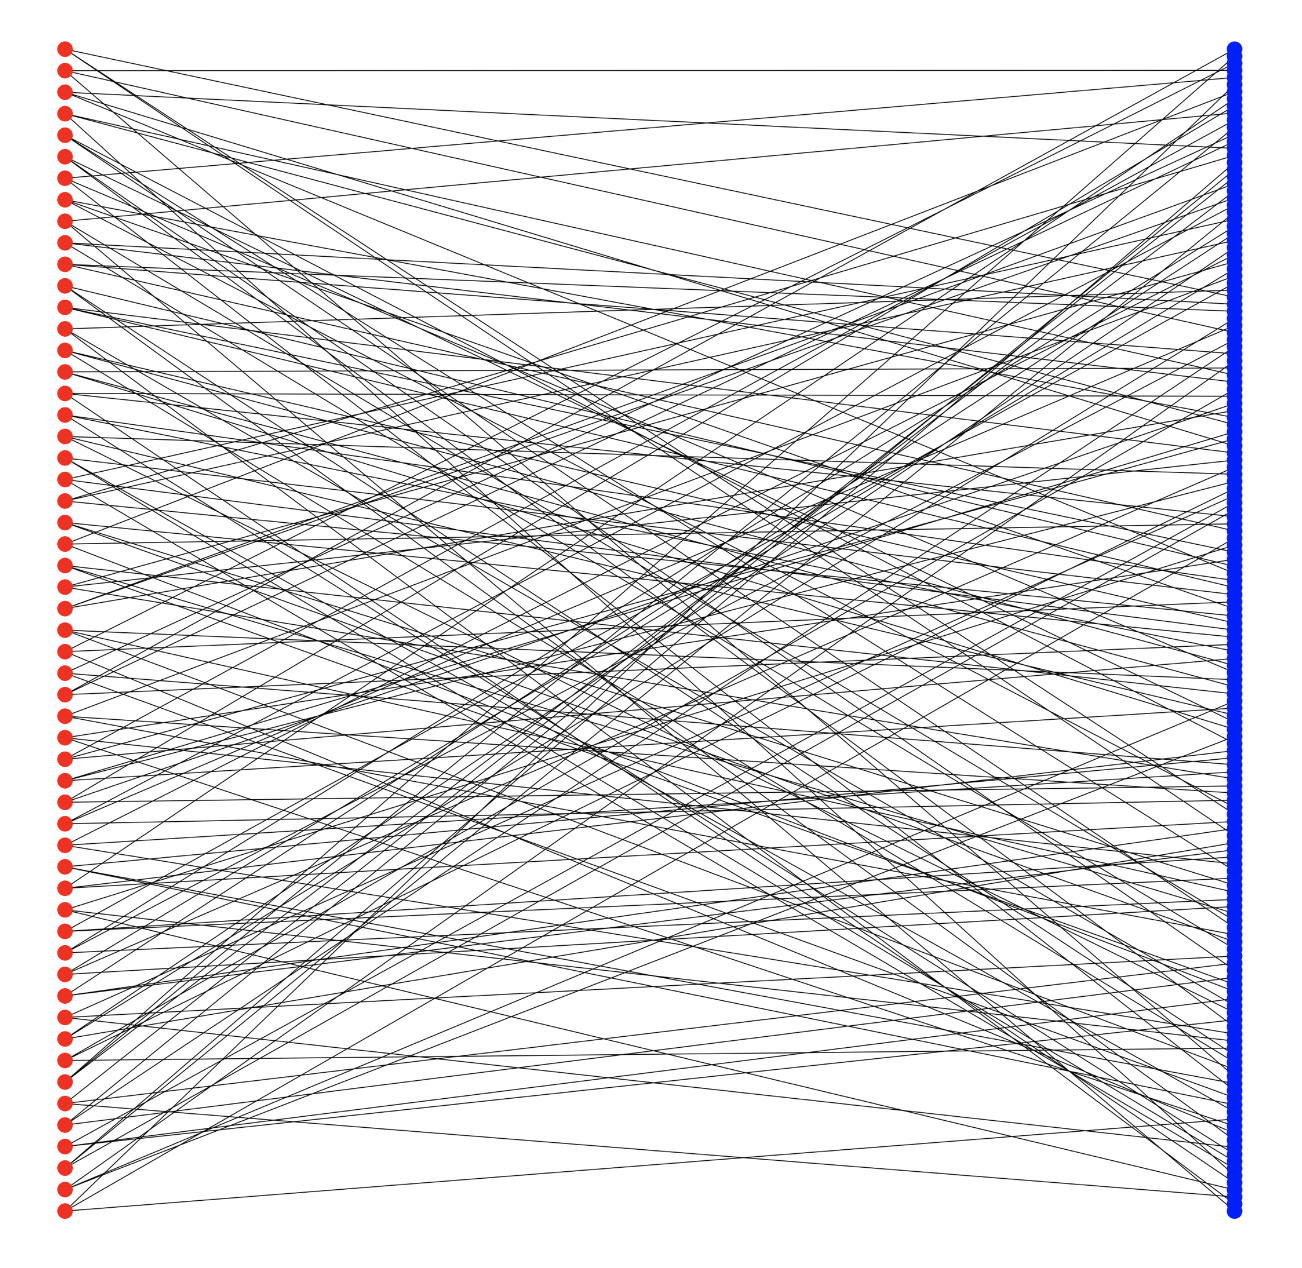
\includegraphics[width=0.95\textwidth]{./img/draw_examples/draw_bipartite.png}
        \caption{Graph produced by \texttt{mg.draw\_bipartite()}. The bipartite structure of the graph is clear, but edge lengths are arbitrary.}
    \end{subfigure}
    \caption{Two visualizations of the \emph{same} graph. This is a graph that resulted from $1:3$ optimal matching. Each graph automatically applies the color-coding of treatment nodes in {\color{red}red} and control nodes in {\color{blue} blue}. Observation IDs/labels may be displayed in either plot by passing \texttt{with\_labels=True}.}
    \label{fig:draw_examples}
\end{figure}


\subsection{Comparison to Other Causal Inference Packages}

Within the Python landscape, there are three existing packages capable of matching for causal inference: \texttt{DoWhy}, \texttt{pymatch}, and \texttt{dame-flame}.
None of them directly use a graph data structure as their primary data structure for conducting the matching procedure, something which makes \texttt{matching} unique. \texttt{matching} also offers the simplest API for iterative matching procedures, as described in \S\ref{subsec:usage}.

Below, I discuss the package in decreasing order of number of stars on its GitHub repo, as a proxy variable for its prevalence among Python data scientists alone (not necessarily a marker of quality!).

\paragraph{\texttt{DoWhy}.} An ``End-to-End Library for Causal Inference'' developed by Microsoft \parencite{dowhypaper}, \texttt{DoWhy} supports matching on a variety of distance metrics, in addition to numerous other methods in the field of Causal Inference (e.g. instrumental variables), and can match the data, build a predictive model for outcomes, and estimate the treatment effect in one shot.
The main drawback of this approach is that matching procedures\footnote{e.g. \texttt{dowhy.causal\_estimators\_propensity\_score\_estimator}} are rigid, ``black-box'' steps that occur as part of treatment effect estimation.
The matching is neither easy to inspect nor flexibly alter without sub-classing \texttt{CausalEstimator}. In short, \texttt{DoWhy} is concerned with estimating treatment effects, and treats the matching procedure as a means to this end, not a process of note in itself. \texttt{matching} could be used to pre-subset the observational data before passing it to \texttt{DoWhy} for further analysis, but the fundamental aims of these packages differ: \texttt{DoWhy} is a high-level API for end-to-end causal inference, whereas \texttt{matching} enables low-level exploration of the matching process.

\paragraph{\texttt{pymatch}.} Purpose-built by researchers working on an observational study \parencite{miroglio_pymatch_2022}, \texttt{pymatch} supports only one distance metric, the propensity score, and the only matching algorithms on offer are ``random'' and ``greedy''; no optimal matching is available. 
The package also lacks support iterative matching procedures.
The codebase is short and succinct, and certainly works well for the specific use-case the researchers intended it for, but it is not feature-complete nor flexible enough to be considered a proper alternative to \texttt{MatchIt} or \texttt{matching}.

\paragraph{\texttt{dame-flame}.} Developed by Duke's \emph{Almost Matching Exactly Lab} \parencite{gupta_dame-flame_2021}, \texttt{dame-flame} implements its two titular matching procedures: DAME \parencite{liu_interpretable_2019} and FLAME \parencite{wang_flame_2021}. As discussed in \S\ref{subsubsec:exactmatching}, these methods extend CEM using machine learning, calculating a weight vector \vec{w} indicating the relative importance of matching on each feature. These algorithms each run fast, and are easier to inspect than \texttt{DoWhy}. However, since these each seek to replicate CEM, and since these are the \emph{only} matching methods provided by \texttt{dame-flame}, this means that \texttt{dame-flame} can only be used with discrete datasets; for users unwilling to coarsen/discretize their data, or users seeking a matching procedure other than DAME and FLAME, \texttt{dame-flame} is not an option. \texttt{matching} does not currently support these algorithms, but they are ``in-the-works''; it can certainly be implemented as a new \texttt{matching.distance.\_Distance} subclass, and their impressive performance merits their inclusion.

\section{Experiments}
\label{sec:experiments}

To demonstrate the use and capabilities of the \texttt{matching} package, I have also conducted the following numerical experiments, which offer practical lessons on parameter-tuning when propensity score matching.

\subsection{Data Generation}

The data were generated according to the following hyperparameters. This follows similar frameworks in the literature, such as those of \textcite{austin_optimal_2011}.
\begin{itemize}
  \item \texttt{size0} ($m$): number of control observations to generate.
  \item \texttt{size1} ($n$): number of treatment observations to generate.
  \item \texttt{p} ($p$): number of features to generate.
  \item \texttt{theta0} ($\theta_0$): the feature means for the control group are distributed as follows:
    \begin{equation}
      \texttt{mean0} = \vec{\upmu}_0 \in \reals^p \sim \mathcal{N}(\theta_0 \cdot \vec{1}_p, 0.25 \cdot \mat{I}_p).
    \end{equation}
  \item \texttt{theta1} ($\theta_1$): the feature means for the treatment group are distributed as follows:
    \begin{equation}
      \texttt{mean1} = \vec{\upmu}_1 \in \reals^p \sim \mathcal{N}(\theta_1 \cdot \vec{1}_p, 0.25 \cdot \mat{I}_p).
    \end{equation}
  \item \texttt{rho} ($\rho$): the feature covariance matrix (for both groups) is set as follows:
    \begin{equation}
      \texttt{K[i][j]} = \mat{\Sigma}_{i j} = \begin{cases}
        1    & \text{ if } i = j \\
        \rho & \text{ otherwise.}
      \end{cases}
      \label{eqn:dgm_K}
    \end{equation}
\end{itemize}
We then draw features
\begin{equation}
  \{ \vec{x}_{C_j} \}_{j=1}^{m} \sim \mathcal N(\vec{\upmu}_0, \mat{\Sigma}), \text{ and }
  \{ \vec{x}_{T_i} \}_{i=1}^{n} \sim \mathcal N(\vec{\upmu}_1, \mat{\Sigma}).
\end{equation}
The treatment assignments \texttt{z} were deterministically set according to which mean vector the rows were drawn from. For each set of hyperparameters (as listed above), 30 datasets were generated, and summary statistics to judge the ``quality of matching'' were averaged across these trials.

The two experiments each test the robustness and suitability of varying calipers with regards to a strenuous data setting: one of increasing correlation between the features, and one of increasing imbalance of the features (between treatment and control groups).

In each experiment, propensity scores were fit using standard Logistic Regression, and then optimal $1:1$ matching was conducted, meaning the maximum size of the matched subset would be 500 observations. Each experiment varies one hyperparameter against caliper values $c \in \{0.05, 0.10, 0.15, \ldots, 0.50\}$. To assess the balance of the matched subset, we record the mean \emph{absolute} standardized mean difference of the features in the matched subset; out of practical considerations, we also record the proportion of treatment observations matched $\in [0, 1]$.

\subsection{Experiment 1: Caliper vs Imbalance.}
This experiment seeks to investigate the practical truth of the ``Paradox of Propensity Score Matching'' \parencite{king_why_2019}. The Paradox suggests that matching quality could (not necessarily \emph{must}) deteriorate as the imbalance between the treatment and control groups decreases; this is a logical extrapolation from that earlier-noted fact that when $\mat{X} \perp \vec{z}$, the classifier will assign a constant propensity score to all observations.

For this experiment, we hold constant \texttt{size0=750}, \texttt{size1=250}, \texttt{p=5}, \texttt{theta0=0}, \texttt{rho=0} for all simulated data.
Then, we vary $\texttt{theta1} = \theta_1 \in \{0, 0.1, 0.2, \ldots, 1\}$.

\begin{figure}[h!]
  \centering
  \begin{center}
    \begin{subfigure}[t]{0.49\textwidth}
        \centering
        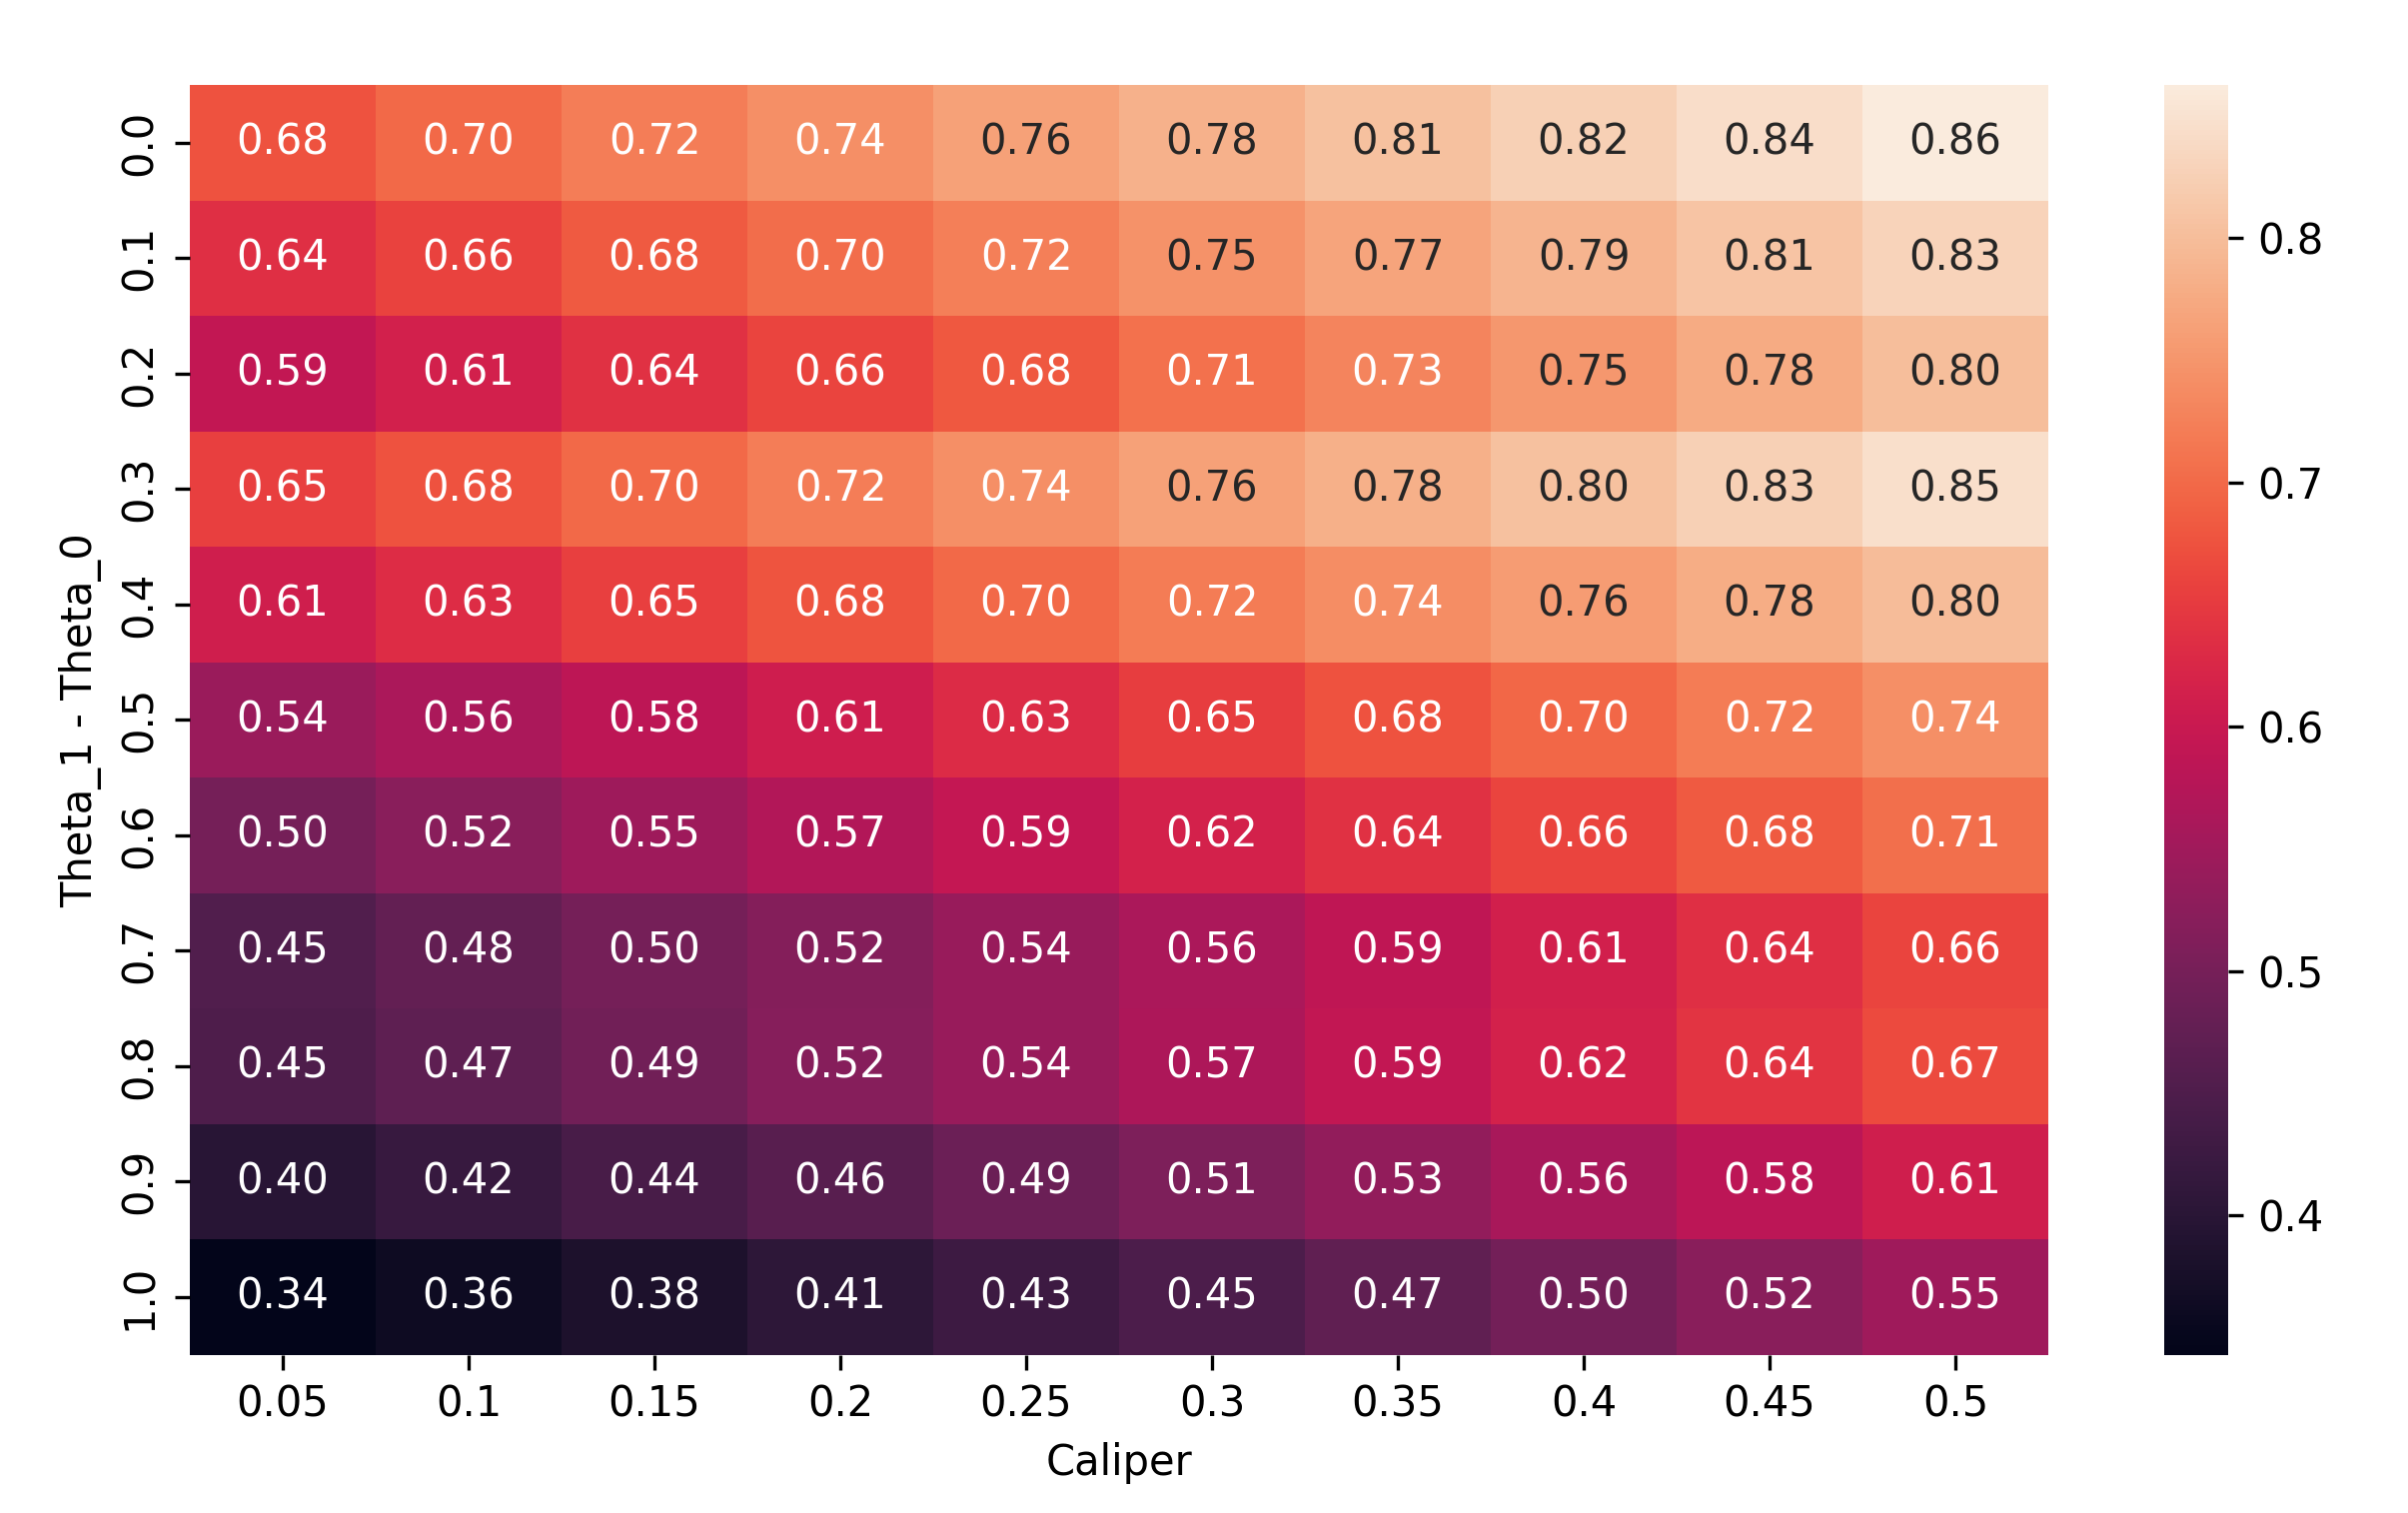
\includegraphics[width=\textwidth]{./img/output30/caliper_vs_imbalance_big/plots/theta1_caliper_prop1_match.png}
        \caption{Proportion of treatment observations matched}
        \label{subfig:exp1_nmatch}
    \end{subfigure}
    \begin{subfigure}[t]{0.49\textwidth}
        \centering
        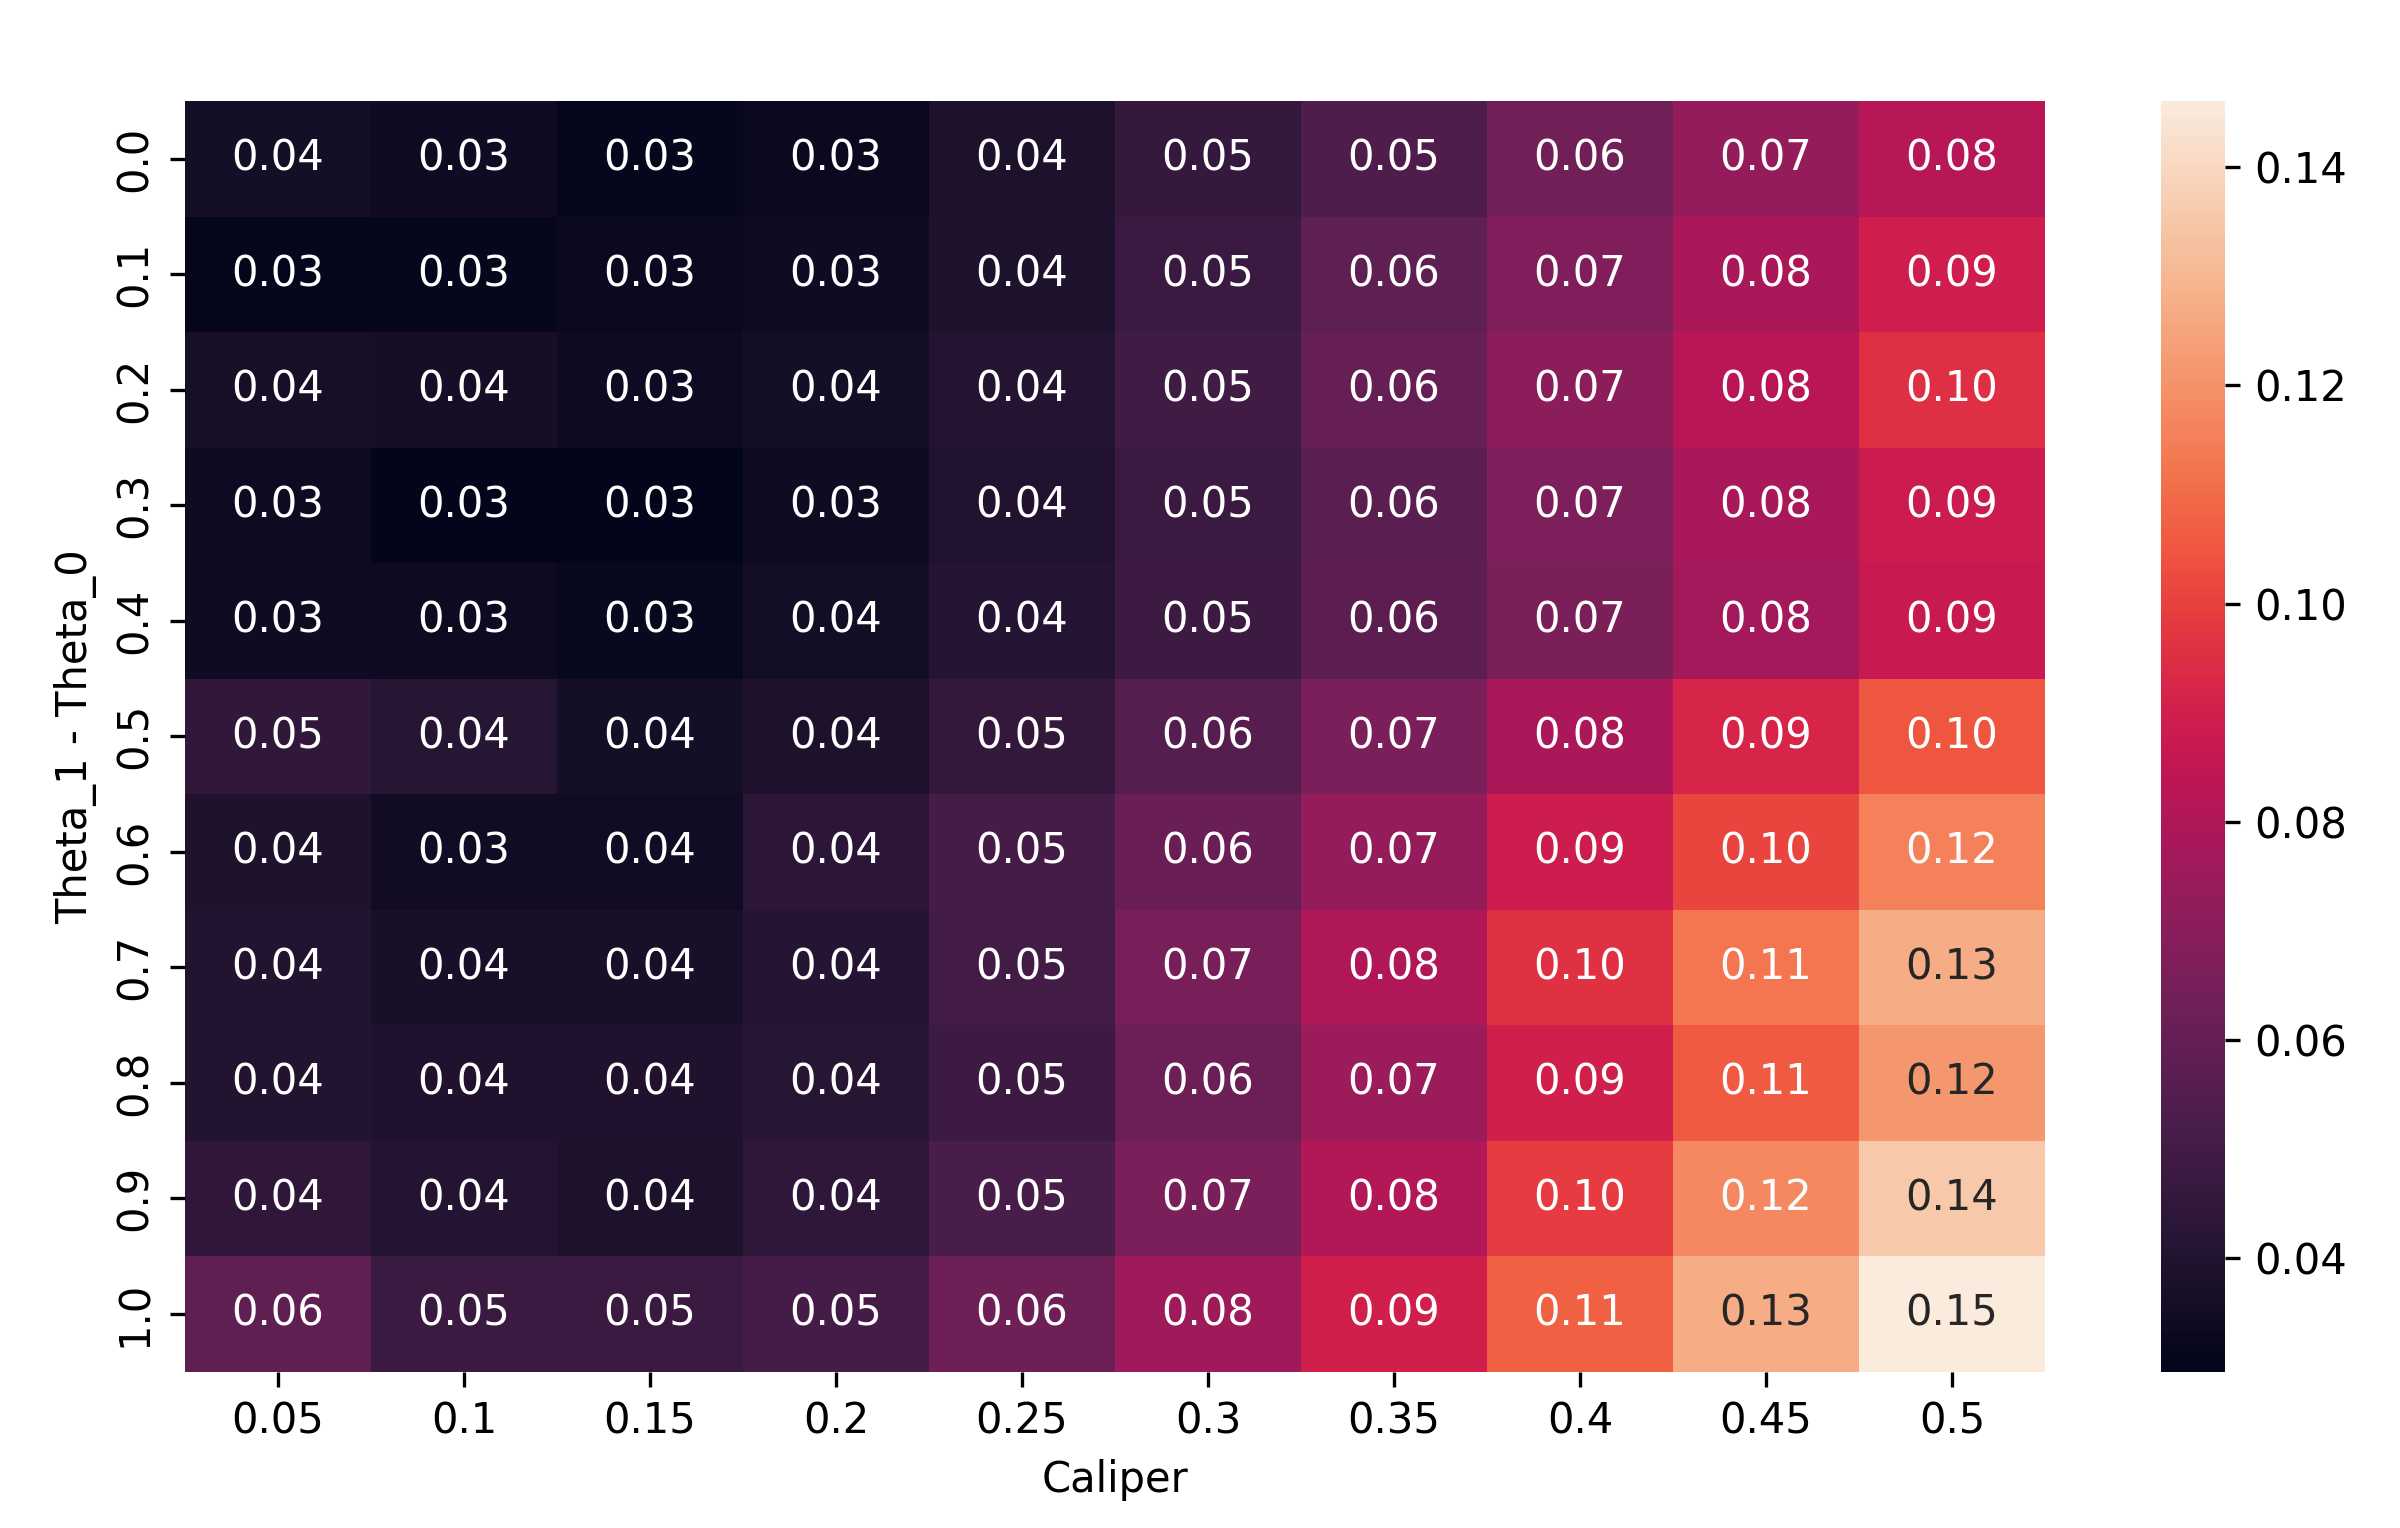
\includegraphics[width=\textwidth]{./img/output30/caliper_vs_imbalance_big/plots/theta1_caliper_mean_abs_smd.png}
        \caption{Mean absolute standardized mean difference}
        \label{subfig:exp1_mean_abs_smd}
    \end{subfigure}
    \caption{$\rho$ is varied from $0.0$ to $0.8$ in increments of $0.1$ \emph{down} the $y$-axis. $c$ is varied from $0.05$ to $0.5$ in increments of $0.05$ along the $x$-axis.}
  \end{center}
\end{figure}

\paragraph{Analysis of Subfigure~\ref{subfig:exp1_nmatch}.} Of course, the proportion of treatment observations matched is monotonically increasing in $c$. This heatmap makes clear that when heterogeneity of the features is too large (even just a single standard deviation apart), the proportion of treatment observations matched may decrease substantially when using the same caliper $c$ (here, we see a decrease of 50\% for $c = 0.05$).
\paragraph{Analysis of Subfigure~\ref{subfig:exp1_mean_abs_smd}.} First, we note that the mean absolute standardized mean difference is nearly constant down the leftmost column (with calipers of $c=0.05$); the cost of imbalance was primarily paid in the size of the matched subset. In fact, the test statistics increase very little with imbalance for most values of $c$; only for $c = 0.45$ and $c = 0.50$ is the increase in imbalance from $\theta_1 = 0$ to $\theta_1 = 1$ greater than $0.05$. This suggests some robustness of the caliper, for normally distributed means that differ by no more than a standard deviation of the data. Moreover, we do not observe the Paradox; the propensity score matching performs very well when $\theta_0 = \theta_1 = 0$. This does not disqualify the Paradox -- it could certainly happen -- it just was not present in this multivariate Normally distributed data.

Finally, we should note that the value of $c$ minimizing the test statistic was not necessarily $0.05$ in all cases; in fact, almost all datasets saw equal or better balance achieved by $c = 0.10, c = 0.15,$ and $c = 0.20$. This underscores the importance of thorough parameter search, as well as balance assessment.

\subsection{Experiment 2: Caliper vs Correlation.}
This experiment seeks to assess the impact that varying correlation among the features has on selection of an optimal caliper. Specifically, it hypothesizes that the optimal choice of caliper will vary significantly as correlation changes; this would be in line with results of the aforementioned \textcite{austin_optimal_2011}.

For this experiment, we hold constant \texttt{size0=750}, \texttt{size1=250}, \texttt{p=5}, \texttt{theta0=0}, \texttt{theta1=1} for all simulated data.
Then, we vary $\texttt{rho} = \rho \in \{0, 0.1, 0.2, \ldots, 0.8\}$.

\begin{figure}[h!]
  \centering
  \begin{center}
    \begin{subfigure}[t]{0.49\textwidth}
        \centering
        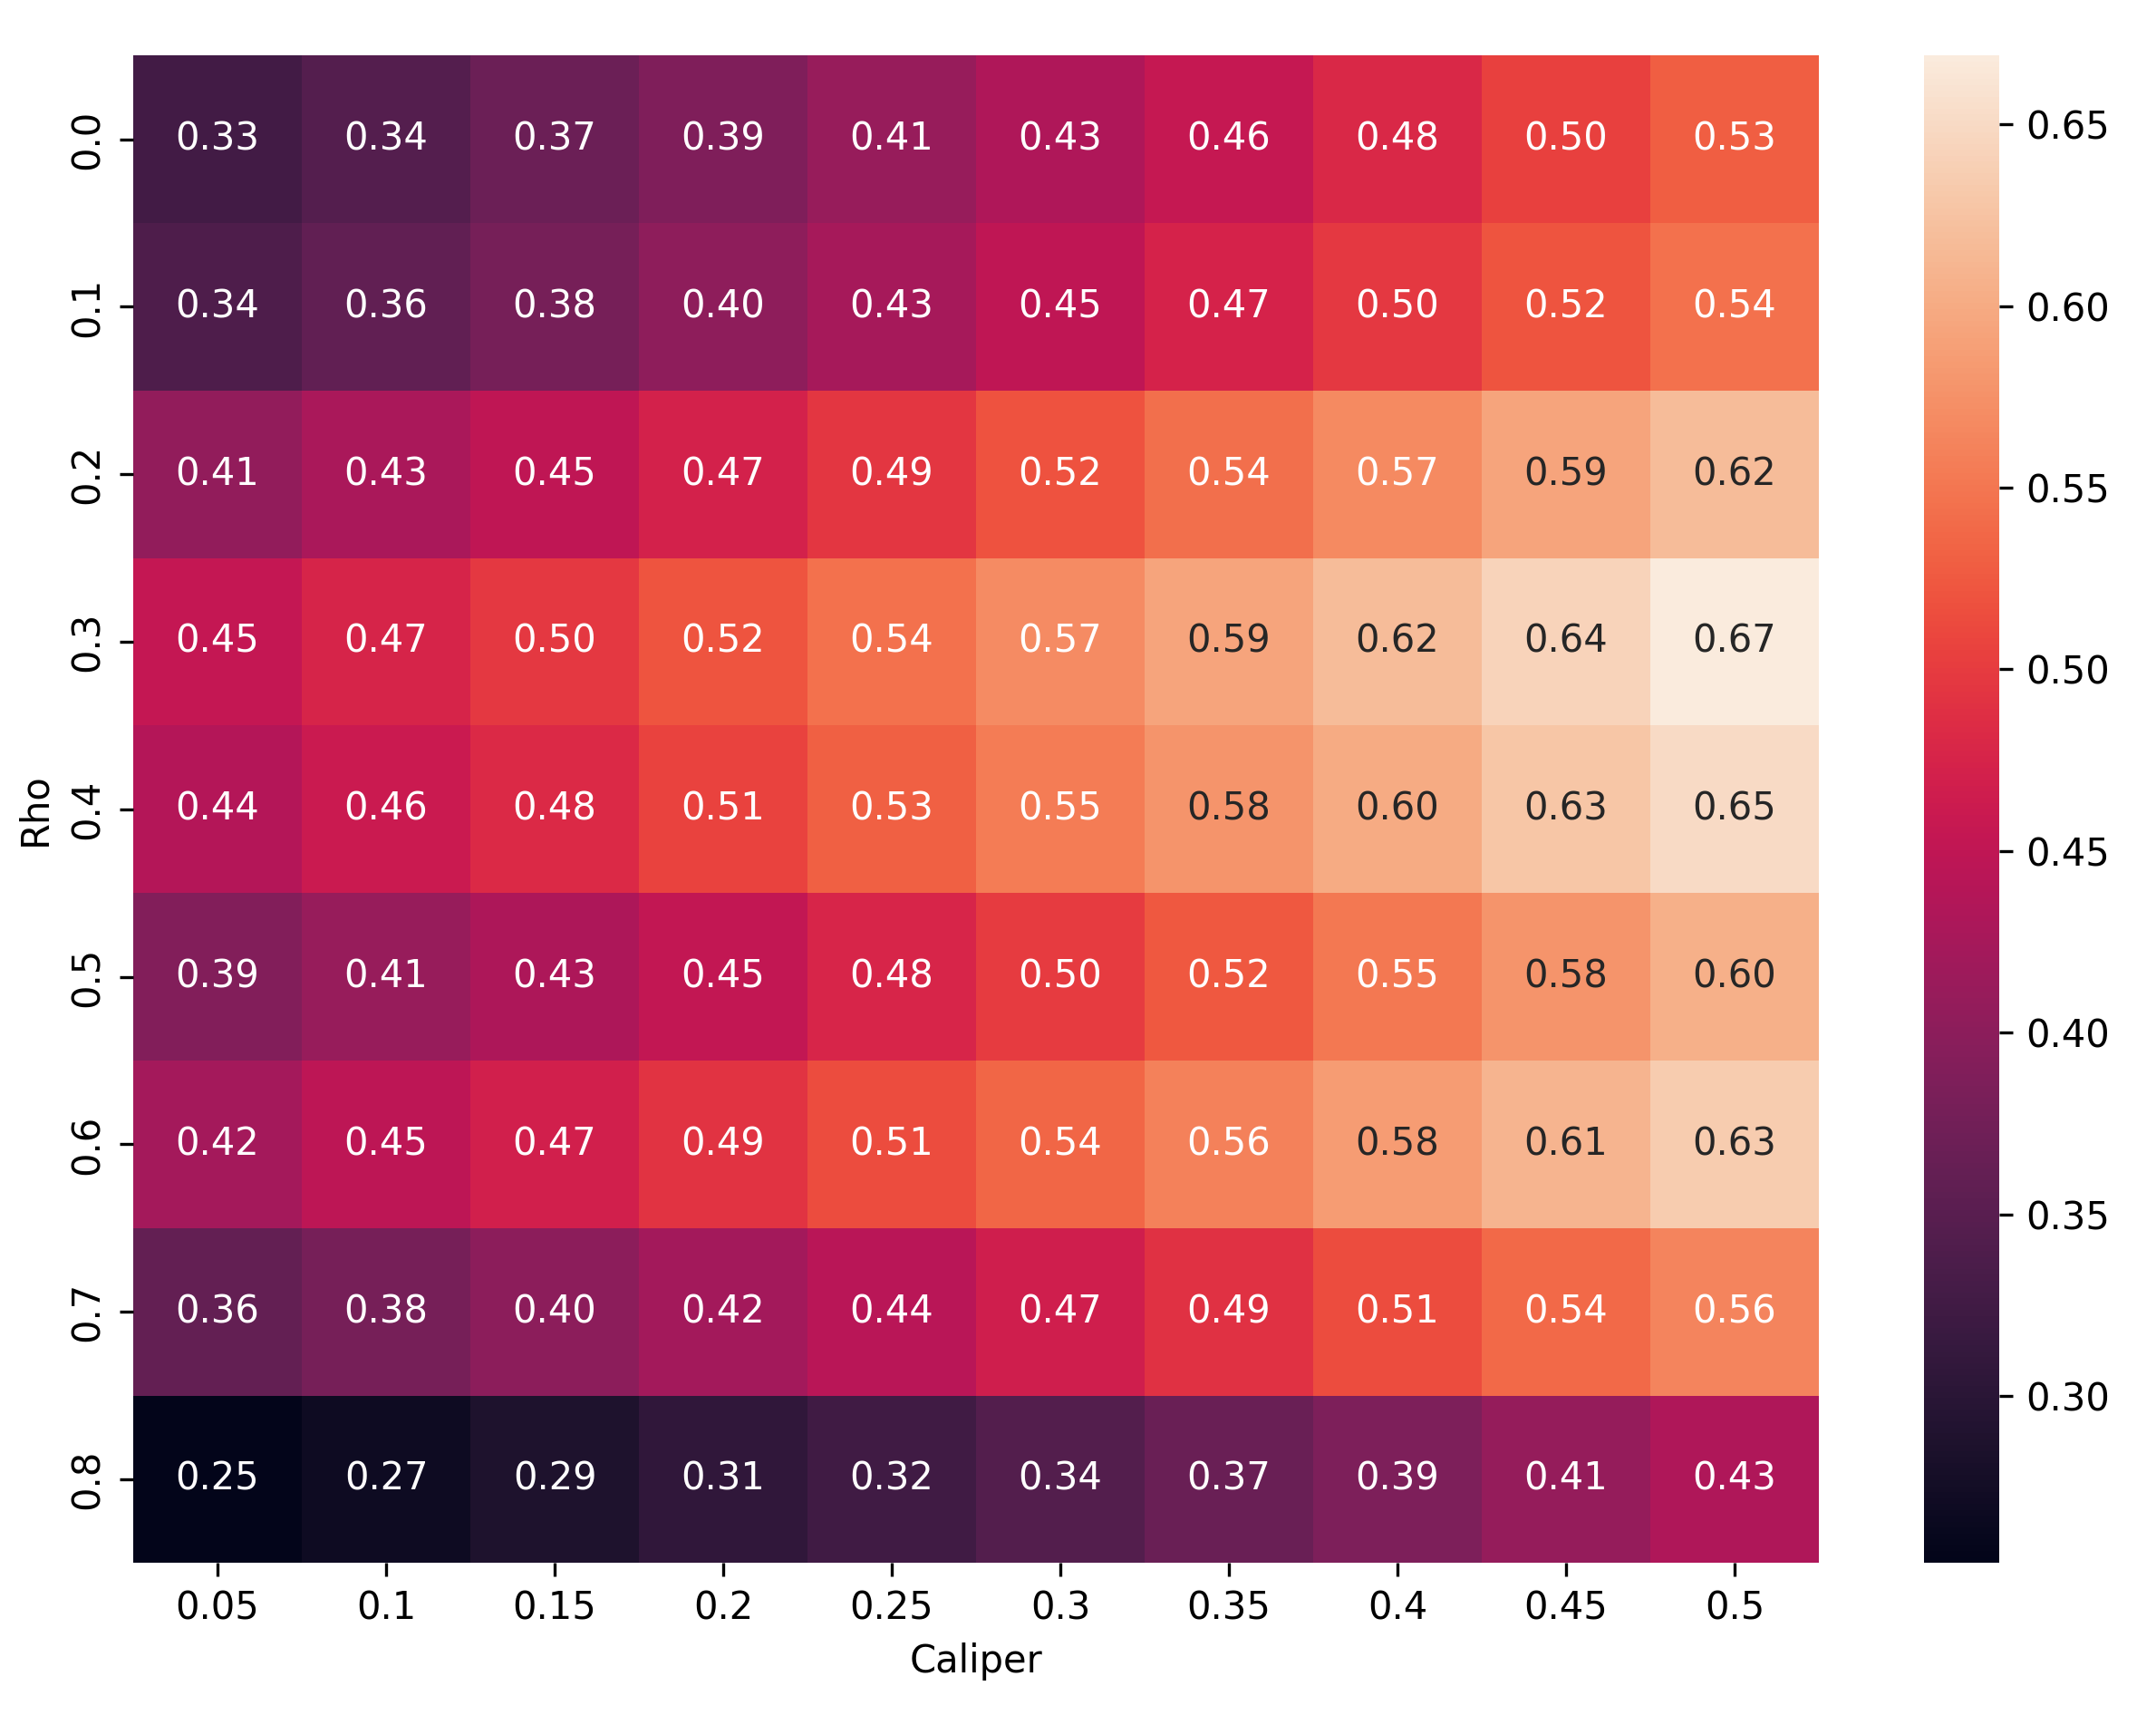
\includegraphics[width=\textwidth]{./img/output30/caliper_vs_correlation_big/plots/rho_caliper_prop1_match.png}
        \caption{Proportion of treatment observations matched}
        \label{subfig:exp2_nmatch}
    \end{subfigure}
    \begin{subfigure}[t]{0.49\textwidth}
        \centering
        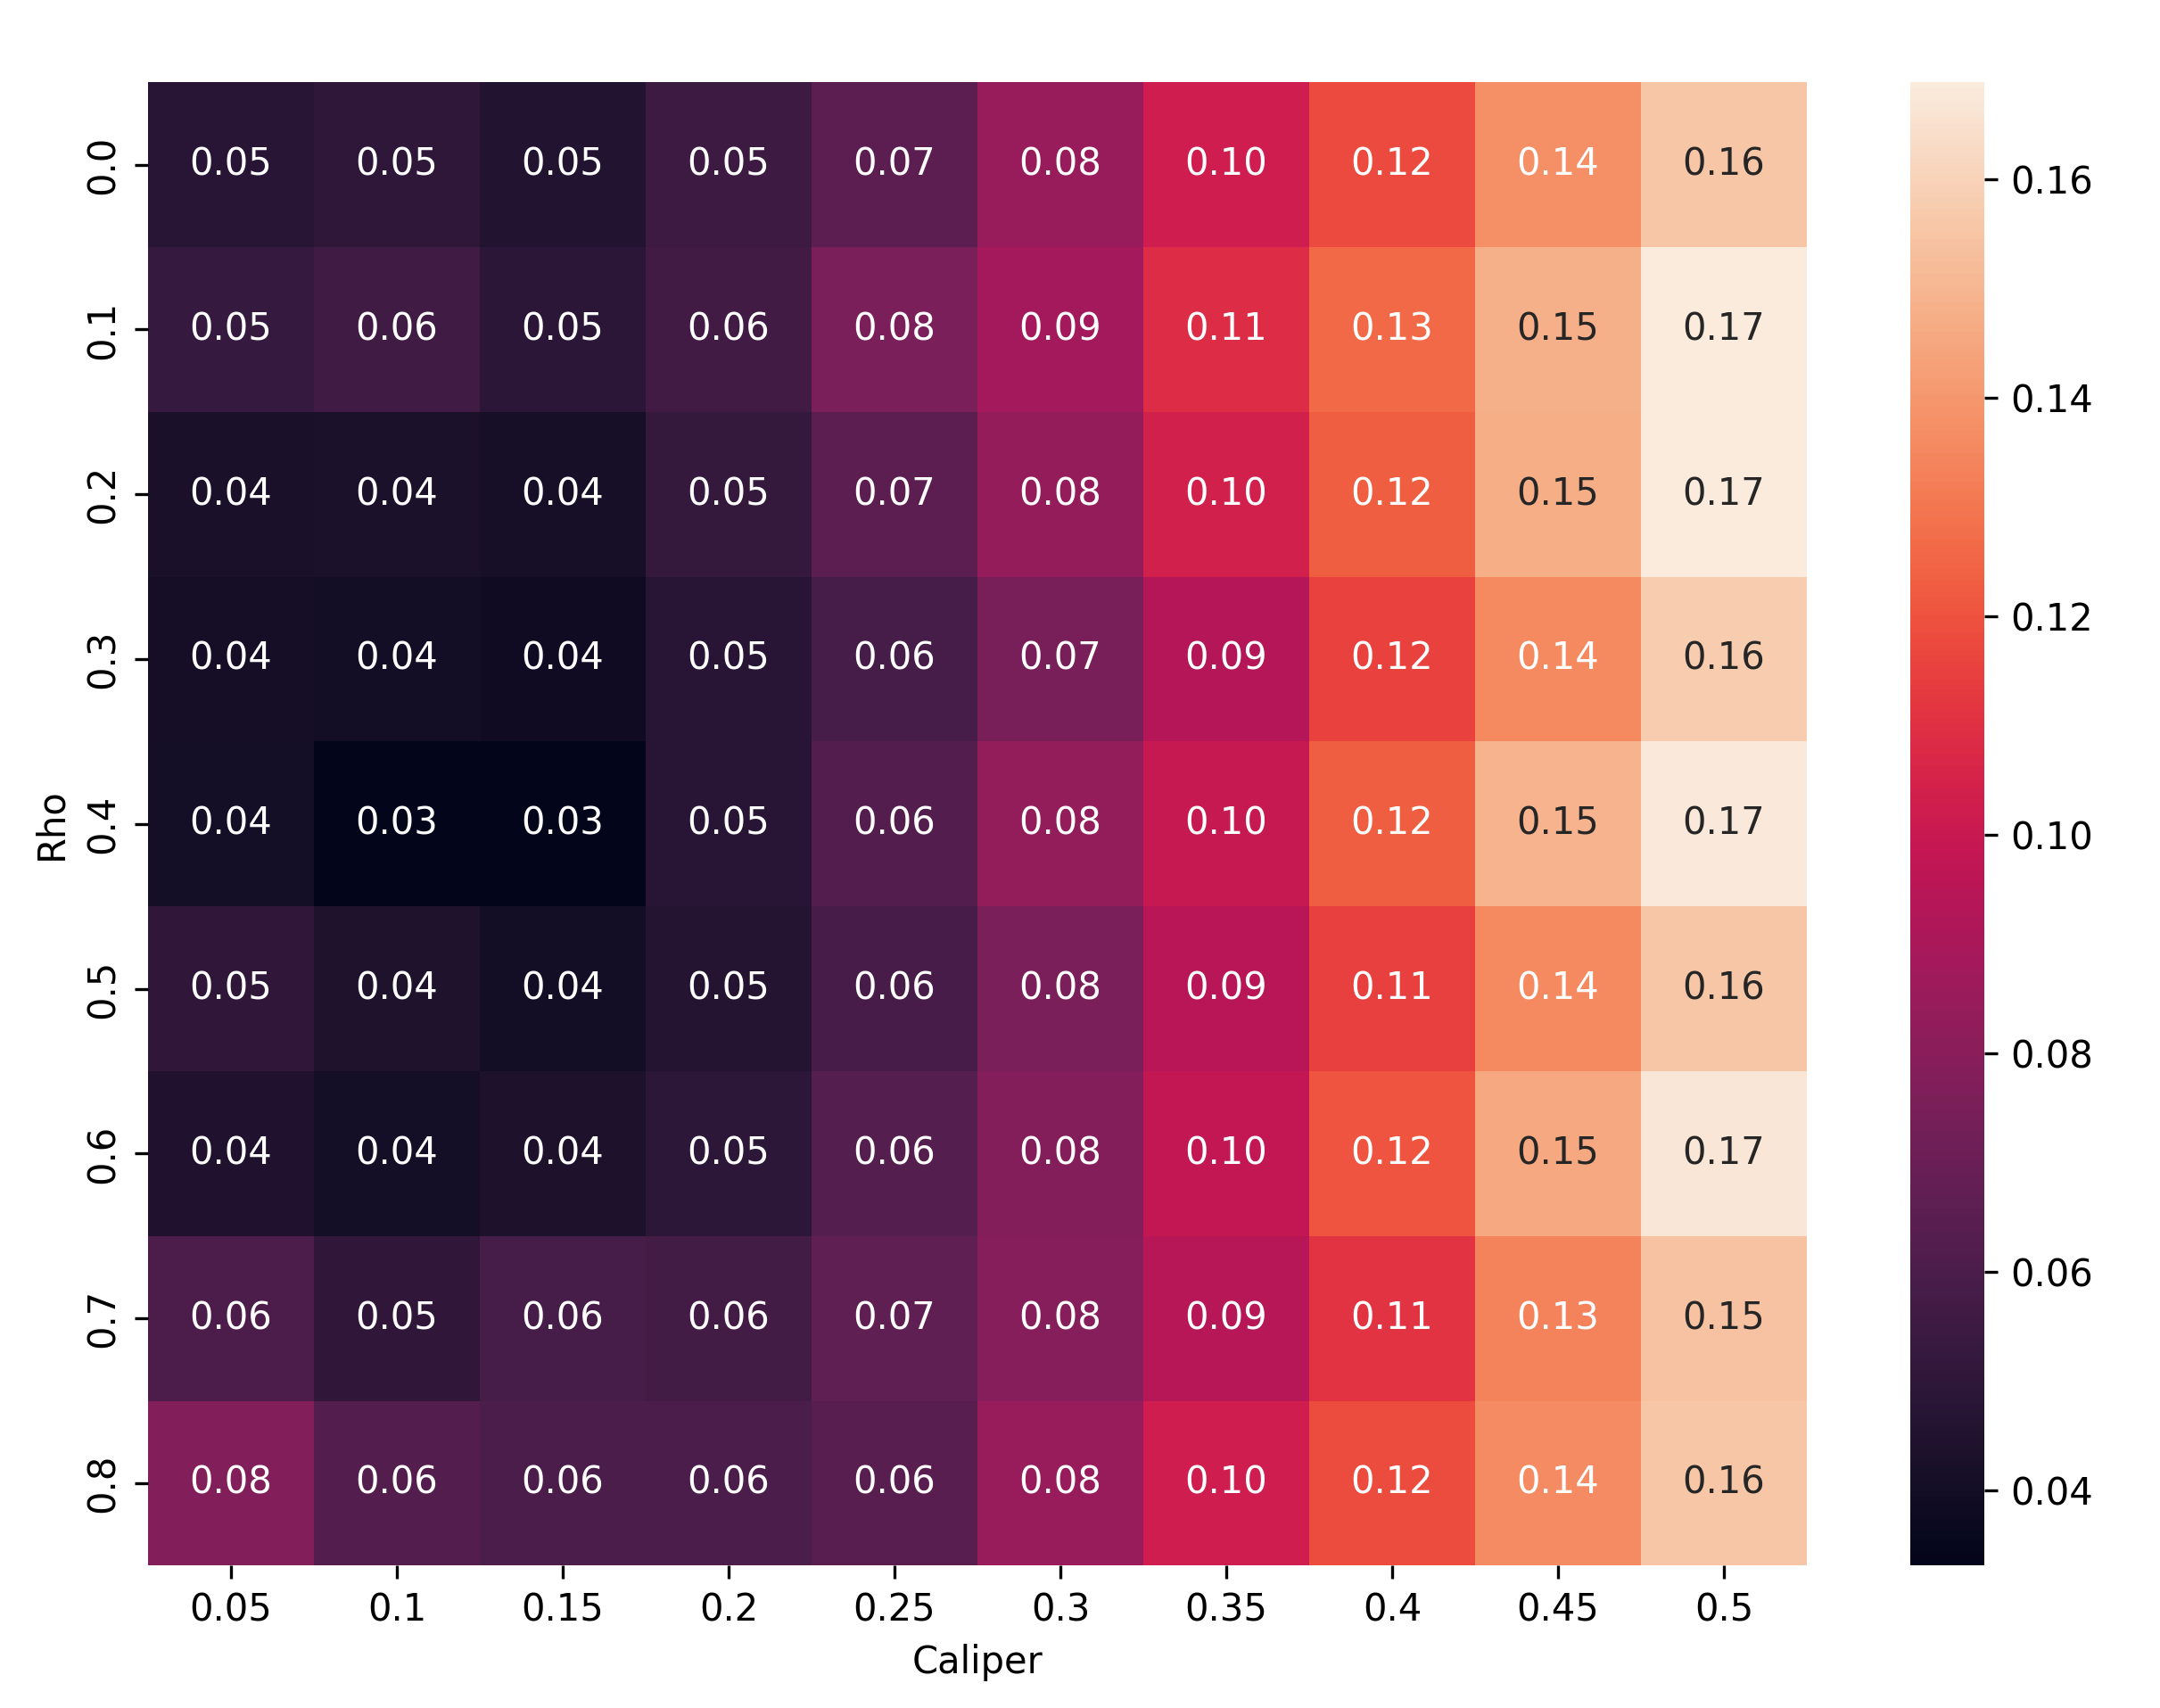
\includegraphics[width=\textwidth]{./img/output30/caliper_vs_correlation_big/plots/rho_caliper_mean_abs_smd.png}
        \caption{Mean absolute standardized mean difference}
        \label{subfig:exp2_mean_abs_smd}
    \end{subfigure}
    \caption{$\theta_1$ is varied from $0.0$ to $1.0$ in increments of $0.1$ \emph{down} the $y$-axis. $c$ is varied from $0.05$ to $0.5$ in increments of $0.05$ along the $x$-axis.}
    \label{fig:exp2}
  \end{center}
\end{figure}
\paragraph{Analysis of Subfigure~\ref{subfig:exp2_nmatch}.} There is not much discernable pattern in the proportion of observations matched with respect to $\rho$ until $\rho=0.8$, which performs very badly. Interestingly, moderate values of $\rho$ (e.g. $\rho=0.3$) afforded the highest proportion of treatment observations, in some cases much higher than in the case of independent features ($\rho = 0$).
\paragraph{Analysis of Subfigure~\ref{subfig:exp2_mean_abs_smd}.} There is again not much pattern in the data with respect to $\rho$. This time, even $\rho=0.8$ performs adequately; it has the highest mean absolute standardized mean difference for most values of $c$, but it is generally not ``much worse'' than any of the other cases. In fact, we find that the test statistic is minimized at modest values of $\rho$ (e.g. $\rho=0.3$); this is no doubt correlated with the high-proportion of treatment group observations matched for those same values of $\rho$.

This analysis suggests that propensity score matching was able to produce high-quality matches even when the data generating model consisted of highly correlated features. This is in line with results presented in other research, such as \textcite{austin_optimal_2011}.

\section{Conclusion}

\texttt{matching} was developed with the real-world researcher responsibilities of tuning their matching process's parameters and assessing its balance in mind. By allowing for constant access to visual and numerical diagnostics throughout the procedure, the user has instant access to diagnostics informing how they should tune their hyperparameters, such as the regularization of the propensity scoring model, or the caliper of matching.
Perhaps the most common theme present throughout all numerical investigation and comparisons of matching methods is the extreme data-dependence of the match quality; by offering a simple-to-use, plug-and-play framework for specifying matching procedures, users are empowered to explore match quality in great detail.

The graph-centric nature of \texttt{matching} also affords many advantages: the third-party dependency (\texttt{networkx}) which handles graph initialization and manipulation is highly memory-optimized.
Since we only need to keep track of the \emph{distance between} treatment observations and control observations (and furthermore dropping those greater than a specified \texttt{max\_distance}), we can precisely represent the similarity between even large datasets, avoiding multiplicative growth of necessary space.

Finally, it is important to remember that diagnostic checks must be chosen to suit the situation. In the case of the experiments conducted in \S\ref{sec:experiments}, mean absolute standardized mean difference was useful because we knew the true difference between $\theta_1$ and $\theta_0$; in practice, this quantity is unknown. As such, researchers should use robust methods of balance assessment; for example, checking for convergence of higher-order moments, or using density-based metrics such as those of \textcite{zhu_kernel-based_2018}. But even then, one cannot possibly hope to analyze the balance of the \emph{unobserved} confounding features; for these, we are only promised balance \emph{on average}. Future research in matching could certainly explore the integration with other causal inference methods, such as the difference-in-differences method or the usage of instrumental variables, which seek to account for the effects of unobserved features.


\cleardoublepage
\section*{Addenda}
\addcontentsline{toc}{section}{Addenda}

\begin{itemize}
  \item Extensive documentation for the \texttt{matching} package can be found on the GitHub at this \href{https://github.com/jackpotrykus/propensity-score-matching-thesis/blob/d47cd58ae7c6cd3fc8a5afc940212e2674d6e7ba/docs/matching.pdf}{link}. This PDF documents every class, function, and method available to the user in great detail, and will serve as a very useful tool for anyone looking to learn how to use the package.
\end{itemize}



% NOTE: SEE LINK BELOW
% https://tex.stackexchange.com/questions/8458/making-the-bibliography-appear-in-the-table-of-contents
% Special handling of bibliography awaits!!
\cleardoublepage
\phantomsection
\addcontentsline{toc}{section}{Bibliography}
\printbibliography


\end{document}
